
%%
% Είδος: διπλωματική στα αγγλικά
\documentclass{uthece-thesis} 


% Πακέτα και ορισμοί που τυχόν χρειάζονται, ανάλογα με το κείμενο της διπλωματικής
\usepackage{algorithm}
\usepackage{algorithmic}

\usepackage[hyphens]{url}
\usepackage{multicol}
\usepackage{multirow}
\usepackage[table]{xcolor}
\usepackage{caption} 
% \captionsetup[table]{skip=10pt}
\usepackage{tikz}
\usepackage{datetime}
\usepackage{ifthen}
\usepackage{hyperref} % Για ενεργά URLs

% Πρόσθετοι ορισμοί, ανάλογα με το κείμενο της διπλωματικής
% typeset source code
\newcommand{\src}[1]{{\tt#1}}

% typeset a backslash
\newcommand{\bkslash}{\symbol{92}}

% Κύρια γλώσσα της διπλωματικής
% μην την τροποποιείτε
\ifgrthesisoption 
    \setlanguage{greek}
\else
    \setlanguage{american} 
\fi

%%%%%%%%%%%%%%%%%%%%%%%%%%%%%%%%%%%%%%%%%%%%%%%%%%%%%%
%%%%%%%%%%%%%   MY PACKAGES %%%%%%%%%%%%%%%%%%%%%%%%%%
\usepackage{listings}
% \usepackage{caption}
\usepackage{subcaption}
\usepackage{mdframed}
\usepackage{siunitx}
\usepackage{pgfplots}
\usepackage{xcolor}


% \usepackage{tikz}

\usepackage{pgfplotstable}
\pgfplotsset{compat=newest}



\lstdefinelanguage{JavaScript}{
  morekeywords={break, case, catch, continue, debugger, default, delete, do, else, false, finally, for, function, if, in, instanceof, new, null, return, switch, this, throw, true, try, typeof, var, void, while, with},
  morecomment=[l]{//},
  morecomment=[s]{/*}{*/},
  morestring=[b]',
  morestring=[b]"
}

\lstset{
  language=JavaScript,
  basicstyle=\ttfamily\fontsize{9}{9}\selectfont,
  keywordstyle=\color{blue},
  commentstyle=\color{green!40!black},
  stringstyle=\color{black},
  frame=none, % Remove frame
  numbers=none, % Remove line numbers
  breaklines=true,
  tabsize=2,
}
%%%%%%%%%%%%%%%%%%%%%%%%%%%%%%%%%%%%%%%%%%%%%%%%%%%%%%
%%%%%%%%%%%%%%%%%%%%%%%%%%%%%%%%%%%%%%%%%%%%%%%%%%%%%%
%%%%%%%%%%%%%%%%%%%%%%%%%%%%%%%%%%%%%%%%%%%%%%%%%%%%%
%% THESIS INFO / ΠΛΗΡΟΦΟΡΙΕΣ ΔΙΠΛΩΜΑΤΙΚΗΣ
%%
% Τίτλος Διπλωματικής Εργασίας στα ελληνικά
	\title{Δημιουργία Μικροϋπηρεσιών σε Δομές Διαδικτύου των Πραγμάτων για Λύσεις Έξυπνης Πόλης\\[0.5em] {\small Μια εφαρμογή παρακολούθησης της ατμοσφαιρικής ποιότητας αξιοποιώντας Apache Kafka και μεθοδολογίες Cloud}}
% Τίτλος Διπλωματικής Εργασίας στα αγγλικά
	\titleEng{Microservices in Internet of Things Infrastructures for Smart City Solutions\\[0.5em] {\small An Event-Driven Air Quality Monitoring Application Utilizing Apache Kafka and Cloud Methodologies}}

 
% Ονοματεπώνυμο φοιτητή στα ελληνικά
	\edef\authorname{Κολοβός Νικόλαος Καλλίνικος}
	\edef\secauthorname{} % κενό αν η εργασία έγινε από έναν φοιτητή
% Ονοματεπώνυμο φοιτητή στα αγγλικά 
	\edef\authornameEng{Nikolaos Kallinikos Kolovos}
	\edef\secauthornameEng{} % κενό αν η εργασία έγινε από έναν φοιτητή
% Ονοματεπώνυμο Επιβλέποντα Καθηγητή στα ελληνικά
	\supervisor{Σταμούλης Γεώργιος}
% Ονοματεπώνυμο Επιβλέποντα Καθηγητή στα αγγλικά
	\supervisorEng{Georgios Stamoulis}
% Φύλλο επιβλέποντα στα ελληνικά 
% Μην το τροποποιείτε για διπλωματική στα αγγλικά
	\edef\supervisorMaleFemale{Επιβλέπων/πουσα}
% Στοιχεία επιτροπής στα αγγλικά
    \edef\supervisortitle{Professor}
    \edef\supervisoraffiliation{Department of Electrical and Computer Engineering, University of Thessaly}
    \edef\memberonename{Charilaos Akasiadis}
    \edef\memberonetitle{Post-Doctoral Researcher}
    \edef\memberoneaffiation{Institute of Informatics and Telecommunications, NCSR 'Demokritos'}
    \edef\membertwoname{Nestor Evmorfopoulos}
    \edef\membertwotitle{Associate Professor}
    \edef\membertwoaffiation{Department of Electrical and Computer Engineering, University of Thessaly}    
% Ημερομηνία υποβολής διπλωματικής
    \newdate{docdate}{04}{02}{2024}
% Ημερομηνία έγκρισης διπλωματικής
    \newdate{docapprovedate}{01}{02}{2024}
% format ημερομηνίας - μην το τροποποιείτε
    \newdateformat{mydate}{\THEDAY-\THEMONTH-\THEYEAR} \mydate
% Τόπος και έτος διπλωματικής στα ελληνικά
	\edef\thesisPlaceDate{Μάρτιος \getdateyear{docdate}}
% Τόπος και έτος διπλωματικής στα αγγλικά
	\edef\thesisPlaceDateEng{March \getdateyear{docdate}}
%
%%%%%%%%%%%%%%%%%%%%%%%%%%%%%%%%%%%%%%%%%%%%%%%%%%%%


\begin{document}

\frontmatter
\maketitle


%%%%%%%%%%%%%%%%%%%%%%%%%%%%%%%%%%%%%%%%%%%%%%%%%%%%%
%% OPTIONAL MATERIAL / ΠΡΟΑΙΡΕΤΙΚΕΣ ΕΝΟΤΗΤΕΣ
%%
% Κατάλογος Σχημάτων προαιρετικά
	\listoffigures % σε σχόλια για μη εμφάνιση
% Κατάλογος Πινάκων προαιρετικά
	\listoftables % σε σχόλια για μη εμφάνιση
% Συντομογραφίες - Αρκτικόλεξα - Ακρωνύμια προαιρετικά
	% Συντομογραφίες - Αρκτικόλεξα - Ακρωνύμια

\newcommand{\abbrev}[2]{#1 \> #2\\ }
\begin{abbreviations}

\begin{tabbing}
%ta 'a' rythmizoun to platos ton dyo stilon
  aaaaaaaaaaaaaaaaa \= aaaaaaaaaaaaaaaaaaaaaa\kill
  \abbrev{IoT}{Internet of Things}
  \abbrev{DevOps}{Software Development and IT Operations}
  \abbrev{D2C}{Device-to-Cloud}
  \abbrev{D2D}{Device-to-Device}
  \abbrev{KRaft}{Kafka Raft metadata mode}
  \abbrev{AMQP}{Advanced Message Queuing Protocol}
  \abbrev{MQTT}{Message Queuing Telemetry Transport}
  \abbrev{TCP}{Transmission Control Protocol}
\end{tabbing}
\end{abbreviations} % σε σχόλια για μη εμφάνιση 
%
%%%%%%%%%%%%%%%%%%%%%%%%%%%%%%%%%%%%%%%%%%%%%%%%%%%%


\mainmatter
%%%%%%%%%%%%%%%%%%%%%%%%%%%%%%%%%%%%%%%%%%%%%%%%%%%%%
%% CHAPTERS / ΚΕΦΑΛΑΙΑ 
%%
    \chapter{Introduction}
\label{chap1}

In recent years, we've seen a significant rise in the use of the internet and technology applications in our daily routines. As we increasingly rely on smartphones and other devices, they are making our lives more convenient, adaptable and in some cases, even safer. A vast array of applications and services are readily available to us, ranging from simple payment and ticket booking systems to high-accuracy GPS maps and numerous other innovative technologies\cite{madakam2015internet}. These technologies can be developed by both leading tech companies and smaller-scale initiatives. Often, these smaller companies or groups of developers aim to implement the well-established and ever-expanding applications of the Internet of Things network. This large network of connected devices is full of potential used to create new solutions that can meet many different needs. From creating smart environments that respond to user behavior\cite{AdvancesinCrowdAnalysis,OverviewofUrbanMobility}, to developing systems that monitor and manage resources for efficiency, such technological innovations are pushing the boundaries of what's possible with IoT technology.

The Internet of Things, commonly referred to as IoT, involves the interconnection of a vast array of devices and services via the internet, with the ultimate aim to orchestrate collective operation.\cite{madakam2015internet,rose2015internet}. This interconnection is designed to generate applications and internet solutions for a wide range of scenarios. Such applications can be found in smart homes, healthcare, agriculture, transportation, energy management, various types of automation and of course, environmental monitoring,\cite{Systematicreview,BIBRI2018230,7562698} which is the focus of our thesis. The broad scope of these implementations aims to enhance the quality of our lives, whether we're discussing large-scale applications or smaller companies seeking straightforward solutions that require internet interconnectivity. The rapid expansion of such applications, coupled with the vast open-source community, can lead to the development of solutions for a wide array of challenges. This is particularly beneficial in certain areas that require more expedient solutions to address their unique local problems. 

Given this local problem-solving approach and the accessibility of smart internet tools provided by IoT, we see the potential for creating widely available applications focused on environmental monitoring and air quality. Air quality and environmental pollution have been major concerns for modern societies and political spectrum in recent years\cite{harper2017environment}. The industrial revolution of the past century, along with the continued use of methods with high carbon and particulate matter footprints, have raised significant concerns, especially in recent years\cite{EuropeanEnvironmentAgency}. From a governmental perspective, particularly in Europe~\cite{EuropeEnvironment}, there has been significant effort to revolutionize industrial production methods to be more efficient and environmentally friendly. Despite these valuable and substantial efforts to reduce air pollution, the problem is far from being fully resolved. These circumstances lead the way for innovative ideas to monitor air quality and pollution in efficient and affordable ways, primarily making them widely available to people concerned about such issues. This is where the extensive capabilities of IoT applications come into play, providing the opportunity to effectively monitor the overall air pollution footprint at a specific location\cite{MobileAirPollutionMonitoring}.

\section{Thesis' Vision}
In our approach, we aim to create a highly interoperable and scalable solution that follows to the core principles of IoT. This is achieved by enhancing the capabilities of the SYNAISTHISI platform with emerging technologies and network protocols increasingly adopted across a broad range of technological infrastructures. SYNAISTHISI platform~\cite{Synaisthisi} initiated the contemporary concept of interconnecting diverse resources for various purposes, complying with the fundamental framework of IoT applications. Its basic idea was the creation of an IoT middle-ware that links a vast array of services, aiming to accomplish any given task: A service hosting platform where various system applications can be developed and operated by users in an easy and scalable manner. Also, the support of multiple protocols across different platforms, systems and services, makes the process of interconnecting elements like sensors, actuators and embedded systems more accessible. This combination of older protocols with newer ones enhances the scalability of our application and facilitates its accessibility for future upgrades and covers a wide spectrum of use cases.

In this regard, we try to bridge our concern and the fundamental right of everyone to access information about the air quality in their living environment. More specifically, there has been significant interest in PM\textsubscript{2.5} particles in the atmosphere, along with general factors like temperature and humidity and their long-term effects on human health\cite{effectofheatandairpollution,RecentInsightsParticulateMatter}. We aim to provide an easy-to-use service for everyone, but most importantly, to encourage technologically savvy individuals to explore the power of existing IoT and open-source infrastructures. With some insight, they can create their own services and conduct their own research on any given problem. This luxury of leveraging existing Cloud infrastructures\cite{ModernComputingParadigms} and adding services to them that can address a wide range of problems is relatively new. Our approach lays the groundwork for innovative methods of developing applications that effectively enhance our lives and keep us informed about existing situations, all while adhering to the principles of the IoT philosophy.

This thesis is embarking on the task of implementing enhancements to an already established platform, which is recognized for its focus on the interoperability features of IoT ecosystems. The enhancements involve the integration of Apache Kafka\cite{WhatIsApacheKafka}, a continuously evolving technology, along with its associated technologies. Our objective is to expand and upgrade the SYNAISTHISI platform, by incorporating an advanced system that propels the process of data transfer and flow to the next level. Apache Kafka, with its event streaming capabilities across various systems, leads the way for fast and responsive IoT applications. Its high throughput, high availability and low latency make it an ideal choice (cf. Sec. \hyperref[event_streaming]{3.2}). With the proper configuration and infrastructure, Kafka can transform small-scale applications into large-scale projects. By incorporating new components, primarily from the Apache project, we can seamlessly interconnect existing protocols and devices with newer ones in an easy and accessible manner. We persist in the fundamental approach of upgradability and expandability, thus ensuring the creation of an IoT platform capable of hosting multiple services and ensuring compatibility with future services across a broad range of use cases.

\clearpage
\section{Contributions}

The contributions of this thesis are summarized as follows:
\begin{enumerate}
\item Design and creation of a comprehensive cloud-based IoT Air Quality monitoring application.
\item Enhanced the SYNAISTHISI platform's event-driven capabilities through the integration of Apache Kafka, Kafka Connect and Schema Registry.
\item Implemented Kafka Connect to interconnect events across multiple protocols, and employed Schema Registry for efficient data validation and message optimization.
\item Develop and configure a high-performance, fault-tolerant and scalable Apache Kafka cluster.
\item Implemented a user-friendly and contemporary web application for real-time air quality data consumption on a live map, utilizing Web-Sockets and React.
\end{enumerate}


\section{Thesis Organization}

The subsequent sections of this thesis are organized as follows: Background, motivation and related work are provided in Chapter 2 (cf. Chap.\hyperref[chap2]{2}), setting the theoretical approach. A detailed analysis of the utilized frameworks and services is presented in Chapter 3 (cf. Chap.\hyperref[chap3]{3}). A comprehensive description of the application's architecture, development process and implementation, including the design of our front-end map, is offered in Chapter 4 (cf. Chap.\hyperref[chap4]{4}). Experimental evaluation and bench-marking of the application, providing an in-depth performance analysis, are the focus of Chapter 5 (cf. Chap.\hyperref[chap5]{5}). Finally, potential future work and expansions, which concludes the thesis with reflections and directions for further research are discussed in Chapter 6 (cf. Chap.\hyperref[chap6]{6}).
    \chapter{Background and Motivation}
\label{chap2}

\section{Environmental Perspective}

In recent decades, there has been significant concern about various forms of pollution on our planet. Air pollution, in particular, has been a major issue for many years, especially in the most industrially advanced countries. A significant consequence of air pollution is the increase in particulate matter in the atmosphere, also known as PM\textsubscript{2.5}. These particles can lead to various health problems, including cardiovascular, respiratory and neurodegenerative diseases \cite{RecentInsightsParticulateMatter}. This, in conjunction with the increasing global temperatures \cite{effectofheatandairpollution}, has shown that even a slight increase in particulate matter pollution can have significant effects. Numerous advanced countries and regions are making strides towards reducing air pollution by not only mitigating 
 \cite{EuropeEnvironment} the factors causing this pollution, but also by enhancing the techniques for monitoring and analyzing air quality.

A prime example of efforts to address this situation is South Korea \cite{IQAir} which is using advanced monitoring and notification technologies to alert its citizens when high levels of air pollution are detected. This includes the involvement of technology companies, like IQAir \cite{IQAir}, which provides high-performance real-time air quality monitoring systems to help combat the country's serious air pollution issues. When air pollution levels surge, citizens are alerted to limit outdoor activities and are advised to use masks capable of filtering particulate matter as a protective measure. Moreover, the initiative to adopt more advanced technologies for tracking the sources and impacts of air pollution has already started to show results, as evidenced by the reduction in the annual PM\textsubscript{2.5} concentration level \cite{AirPollutionControl}, in the past years starting from 2019 to 2022. 

\section{IoT Perspective}

Since such efforts require substantial government and enterprise funds, there has been a push for more accessible, simplified and cost-effective solutions. Internet of Things (IoT), coupled with the widespread impact of the internet on our daily lives \cite{madakam2015internet,ImpactofIoT-BasedSmartCities} over the past decade, has emerged as a central instrument for these accessible solutions. The IoT principles has evolved over the years, finding its place in numerous implementations and applications \cite{ImpactofIoT-BasedSmartCities,7562698}. It utilizes a broad spectrum of device-to-device and device-to-Cloud implementations \cite{IotArchitecture}. Device-to-Device (D2D) communication, devices directly exchange data, optimizing local processing efficiency, but limitations arise in terms of range, scalability challenges and potential security vulnerabilities. Device-to-Cloud (D2C) implementations leverage cloud resources for scalability and cost-efficiency, offering centralized management, but may introduce latency, security concerns and dependence on reliable internet connectivity \cite{CloudIoT}. However, challenges in Device-to-Cloud interactions require careful selection and configuration of the frameworks for a robust implementation. This has paved the way for innovative business models and applications, promoting both technological advancement and economic growth in cities and regions that have embraced this approach in recent years \cite{rose2015internet,7300835}.

A bright example in our local environment in the city of Volos, Greece is GreenyourAir \cite{GreenyourAir}. This IoT-based application employs simple and cost-effective sensors to measure the PM\textsubscript{2.5} concentration level, along with the temperature and humidity, initially in the city of Volos and more recently in other areas as well. It is, of course, utilizing Cloud infrastructure to store and process the real time data coming from affordable sensors. The use of smaller, cost-effective sensors, instead of large stations, facilitates the expansion of the existing network in a cost-efficient way. This approach broadens the availability and accessibility of air quality information to the public. In our thesis, we utilize a portion of their measurements as our data ingestion source, providing real-world data for our application.


\clearpage
\section{Open-source Approach}\label{open_source_approach}
To proceed further, it's essential to understand the significance of open source in general , as the entire expansion of our SYNAISTHISI platform is based on the implementation of open-source tools. Open source projects possess huge influence in the development process of IoT, web applications and projects in general, as they raise a collaborative environment where developers contribute their expertise, leading to robust and innovative solutions \cite{BenefitsofOpen-SourceSoftwareforDevelopers}. This continuous integration accelerates the development process, as issues are identified and resolved swiftly. Furthermore, open source projects provide a lot of learning opportunities for developers through a wide range of levels, while also ensuring transparency, as the source code is openly available for review, improvement and modification. Additionally, transparency enhances trust and allows for the customization of applications to meet specific needs, many large companies \cite{OpenSourceContributorIndex} from various industries to contribute to open source projects, aiming to develop frameworks and services in a more efficient and cost-effective manner. In the IoT field, open source projects have been key in pushing progress, providing many libraries, frameworks and tools \cite{IntelOpensource} that simplify the development process, which combined with the ongoing support for these tools, enhances the scalability and future-readiness. In conclusion, most of the technologies we utilize for our implementation are originated from well-know open-source projects, that provide advanced development tools and frameworks, enabling the appreciation to the significance and value of open source for both small and large scale applications.

\section{SYNAISTHISI Platform}

The primary platform that we are enhancing in this thesis is SYNAISTHISI \cite{Synaisthisi}. It offers the interoperability, scalability and interconnectivity that our application requires. There is a wide variety of supported protocols in the platform, but in this instance, we are primarily focusing on interconnecting Kafka and its associated tools with MQTT and AMQP protocols, through the integrated RabbitMQ brokers that are already supported by the platform. This strategy aligns with the principles outlined in the open-source approach section (cf. Sec. \hyperref[open_source_approach]{2.3}), as we aim to expand our application and integrate it with services that continue to receive support from their development communities, making our project more open and future-proof. In addition, the containerized nature of the services within the SYNAISTHISI platform facilitates an easy way to upgrade the existing infrastructure with Kafka tools and enables a smooth transition to a production environment. Thus, we preserve the IoT perspective of our application and expand it with advanced yet open-source services.

\section{Kafka Integration Large Scale Event Streaming }

Real-time event streaming and processing, involves transmitting events and messages in a distributed system, allowing for reliable, low-latency and high-throughput data transfer \cite{EventStreamingPlatform}. 
Apache Kafka \cite{WhatIsApacheKafka}, is a widely used open-source stream-processing software, designed for large-scale data collection, processing, storage and analysis \cite{KafkaApachePoweredBy}. Since its launch in 2011 \cite{WhatIsApacheKafka}, the top three tech companies - Amazon, Microsoft and Google - have developed their own large-scale event streaming services: Amazon Kinesis \cite{AmazonKinesis}, Azure Event Hubs \cite{AzureEventHubs} and Google Pub/Sub \cite{GooglePub/Sub}, respectively, inspired by the Apache Kafka project. We note that these are paid services on fully managed Cloud provider platforms \cite{CloudNativeApplications}. However, by utilizing Kafka, we gain access to many features typically found in such paid services, along with the large-scale, high-volume and fault-tolerant data ingestion solutions that Kafka offers. Therefore, with the proper configuration and understanding of our application's needs, we can still leverage these capabilities using this widely adopted and contributor-maintained open-source service.
    \chapter{Available Frameworks and Related Work}
\label{chap3}

There have already been made significant studies around the subject pf IoT platforms in general and, more specifically, IoT-based solutions for air quality applications too. Projects like SEMAR \cite{SEMARIoTServer}, which is similar to the SYNAISTHISI platform, aim to develop and maintain their implementations based on IoT principles. Additionally, they provide an interface capable of hosting multiple IoT applications. Papers, such as the one in \cite{SEMARkafka}, aim to extend the SEMAR platform with similar implementations, focusing on developing an air pollution monitoring application that leverages real-time air quality detection and integrates tools from the Kafka ecosystem.
Similarly, in paper \cite{HandlingStreamAirPollutionData}, there is an effort to develop a similar application using various tools developed by Apache and other infrastructures focused on IoT. Our objective differentiates us from these efforts, by aiming to develop a platform that not only accommodates to our air quality requirements by supplying all essential components for an air quality application, but also ensures our platform remains scalable, upgradable and highly available across different hosting environments. We leverage technologies, services, methodologies and configurations originating from the enterprise development business (e.g. data validation, fault tolerance, high throughput) and incorporate them into our IoT and open-source based application.

Progressing, another instance is the development of an air pollution monitoring system with sensors on city buses \cite{sensorsoncitybus}. Another one MoreAir \cite{Low-CostUrbanAir} presents an agile and low-cost urban air pollution monitoring system. These provide some comprehensive solutions and implementations of the innovative idea of installing sensors on city buses to gain a more detailed and focusing on low and accessible cost of such infrastructures. While acknowledging the potential of such efforts, some studies analyze the challenges that they have faced \cite{Howfarhavetheygone}, such as the lack of universal applicability of these implementations for specific purposes. Therefore, a significant part of our focus is on the creation and expansion of an upgradable and expandable platform, able to host IoT based applications similar to air quality monitoring. In this regard, we have avoided developing an overly specialized implementation exclusively for our air quality application. Apart from merely implementing and completing the monitoring task, we also emphasize on the services and tools we are integrating into our platform. We develop and optimize our infrastructure for environmental monitoring, showcasing the re-usability of individual services of our stack across similar infrastructures. We aim to categorize our stack in a way that allows groups and layers of our system to be efficiently maintained and upgraded (cf. Sec. \hyperref[system_overview]{4.1}). Lastly, compared to \cite{SEMARkafka} and \cite{HandlingStreamAirPollutionData}, we place a high priority on implementing and developing services maintained by their contributors and the open-source community. This approach ensures our platform remains future-proof and up-to-date with emerging technologies.

\section{Docker}

The primary development environment utilized in this thesis is Docker~\cite{Docker}. All applications are executed in a containerized environment using the Docker engine, a tool renowned in both the IoT and enterprise markets for its efficiency and reliability. Docker is a platform as a service product that provides the ability for services to run on an operating system level virtualization, as shown in Figure \ref{ComparingContainersandVirtualMachines}. Unlike traditional virtual machines, containerized services such as Docker provide enhanced resource efficiency and uniformity across various environments, making them an optimal choice for modern software development due to their reduced system demands and consistent performance. 

Alternative solutions to Docker are Podman, Containerd and LXC (Linux Containers), all of which offer container runtime services. However, Docker stands out due to its simplicity and large user community, that makes it a more accessible and user-friendly option for developers. By adopting this approach, each individual service is isolated from the others , creating a conducive development environment. This allows developers to focus on their workflow for individual services without the concern of compatibility issues, thereby enhancing productivity and efficiency.

\begin{figure}[htbp]
	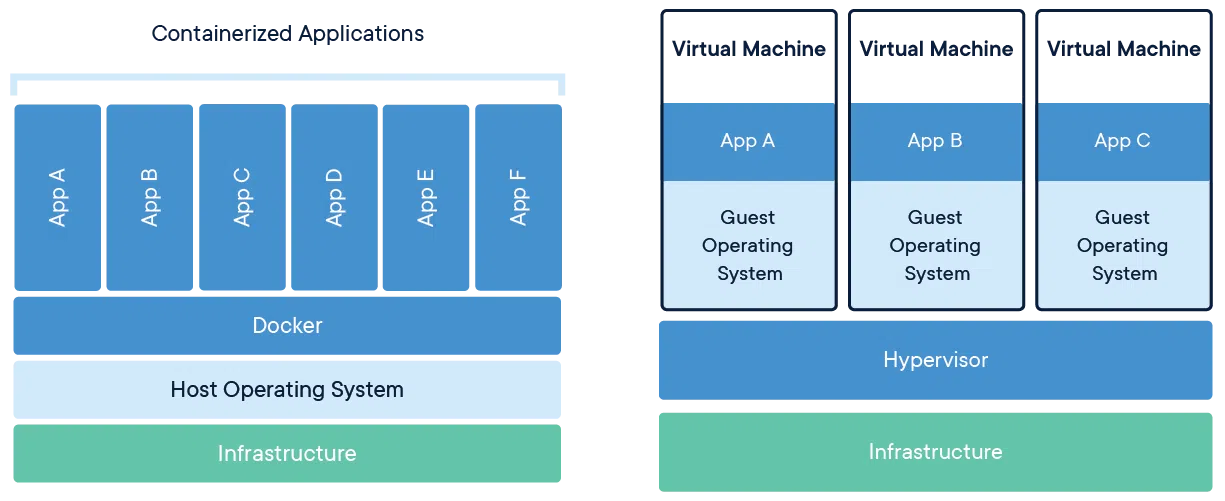
\includegraphics[width=0.75\linewidth]{figures/docker-containerized-and-vm-transparent-bg.png.jpg}
	\centering
	\caption{Comparing Containers and Virtual Machines. \href{https://www.docker.com/resources/what-container/}{[Ref]}}
	\label{ComparingContainersandVirtualMachines}
\end{figure}

\subsection{Docker network}

Containers, as they are referred to, represent these isolated environments. They are interconnected through the advanced Docker network~\cite{DockerNetwork}, which offers a wide array of options and configurations, ensuring high availability for any given setup. This isolation, while also allowing communication between the containers when needed , facilitates the creation of highly scalable and secure applications for future upgrades and optimizations. In contrast to traditional virtualization, Docker images and their associated containers can be incorporated into other applications with minimal configurations, making the project easier to deploy and even adjust in environments that are already deployed.

\subsection{Docker compose}

Docker Compose~\cite{DockerCompose} is a tool that enables the operation of multi-container Docker applications. It serves as the connecting link, providing a simple and organized interface for running multiple containers in conjunction with each other. It offers an ideal environment for both development and smaller scale production applications, allowing developers to have an organized view of their application's configuration, networking and simplifying the development process. Through its interface, developers can coordinate both official and custom images, integrating them into their application as needed. Docker Compose aligns with the DevOps principles, aiming to bridge the gap between the development and the actual functionality of an application.

Today's leading cloud service providers offer near-native support for containerized applications, making Docker tools an excellent choice for managing the development process. This support significantly simplifies the transition from simple IoT implementations to production-level deployments on a cloud provider, making the experience more seamless and intuitive.

\section{Event Streaming}\label{event_streaming}

Event streaming is the process of capturing real time data from a variety of event sources like sensors, devices, gateways, databases and other cloud services. Apache Kafka \cite{WhatIsApacheKafka} is a relatively recent technology that introduces the concept of event streaming to the cloud community. The main flow scheme utilized here is publish/produce, store, subscribe/consume. This model is versatile and can be applied to nearly any type of cloud communication , its primary function being to handle large amount messages per second.

\subsection{Apache Kafka}

Apache Kafka provides low latency, high throughput, scalability and high availability. Kafka enables the use of high-volume real-time data transfer with low latency and provides temporary storage for short-term usage. In contrast, the conventional database model requires all produced data to be first stored in the database before it can be used for any given task. Kafka can be viewed as a cloud cache, offering high availability and low latency , which makes it an excellent choice for real-time event streaming applications. Event streaming is leveraged across a wide spectrum of use cases, including activity tracking for real-time insights, processing data in real-time for immediate decision making, providing low latency and fault-tolerant messaging for critical systems , monitoring operational data to maintain system health and aggregating logs for efficient analysis and troubleshooting.

\subsection{Events}
\label{events}
Events or event records are the messages that contain the information about an actual event that happened (in a structured manner) and they are the main way of reading and writing data to Kafka. An event mainly consists of a key, a value and a timestamp.
Each event within the same topic is distinguished by a unique key. The key determines how these events are distributed across different partitions (cf. Sec. \hyperref[kafka_topics]{3.2.4} \hyperref[kafka_partitions]{ 3.2.5}).
The value is the actual data that is distributed and varies from simple text, to JSON file and even more complex formats like Avro \cite{Avro}, that are encoded properly and stored in the Kafka topics. The timestamp contains information about the time that each event took place.

In the following example, the key 'MqttSensor1' uniquely identifies the source of the data produced or consumed by a Kafka topic. The value 'Mqtt sensor 1 measured $25^{\circ}C$' represents the actual data recorded and the timestamp 'Jul. 15, 2022 at 12:56 a.m.' indicates when this measurement was taken.
\begin{itemize}
    \item Key: 'sensor1'
    \item Value: 'Sensor 1 measured 22.5 \si{\celsius}'
    \item Timestamp: '2/3/2024, 3:14:23 PM'
    % \item Optional metadata
\end{itemize}

\subsection{Brokers}
Brokers serve as the primary infrastructure where data is temporarily stored for subsequent processing, before being pushed for long-term storage. Brokers are organized into clusters, allowing for multi-broker and multi-cluster setups. We do not delve into multi-cluster implementations, since they are primarily used in large-scale multi-region enterprise applications \cite{MultiClusterImplementation}. The complexity and operational overhead of managing multiple clusters is not justifiable for most IoT applications, since our single-cluster implementation meets the requirements for high throughput, fault-tolerance and low latency. 

In the past, Kafka was utilizing Zookeeper \cite{zookeeper} to orchestrate the communication between the Kafka broker nodes and the metadata management. But now, a new protocol called KRaft(Kafka Raft metadata mode) \cite{Kraft} has been implemented to act as the new quorum controller and has a more direct connection to all the Kafka nodes. Nodes can function as a controller, a broker, or both, as depicted in Figure \ref{Kafka_Internals_052}. Controller nodes , deployed as Kafka images, play a crucial role in storing all the necessary metadata for managing the distribution and synchronization of data across the broker nodes.

\begin{figure}[htbp]
	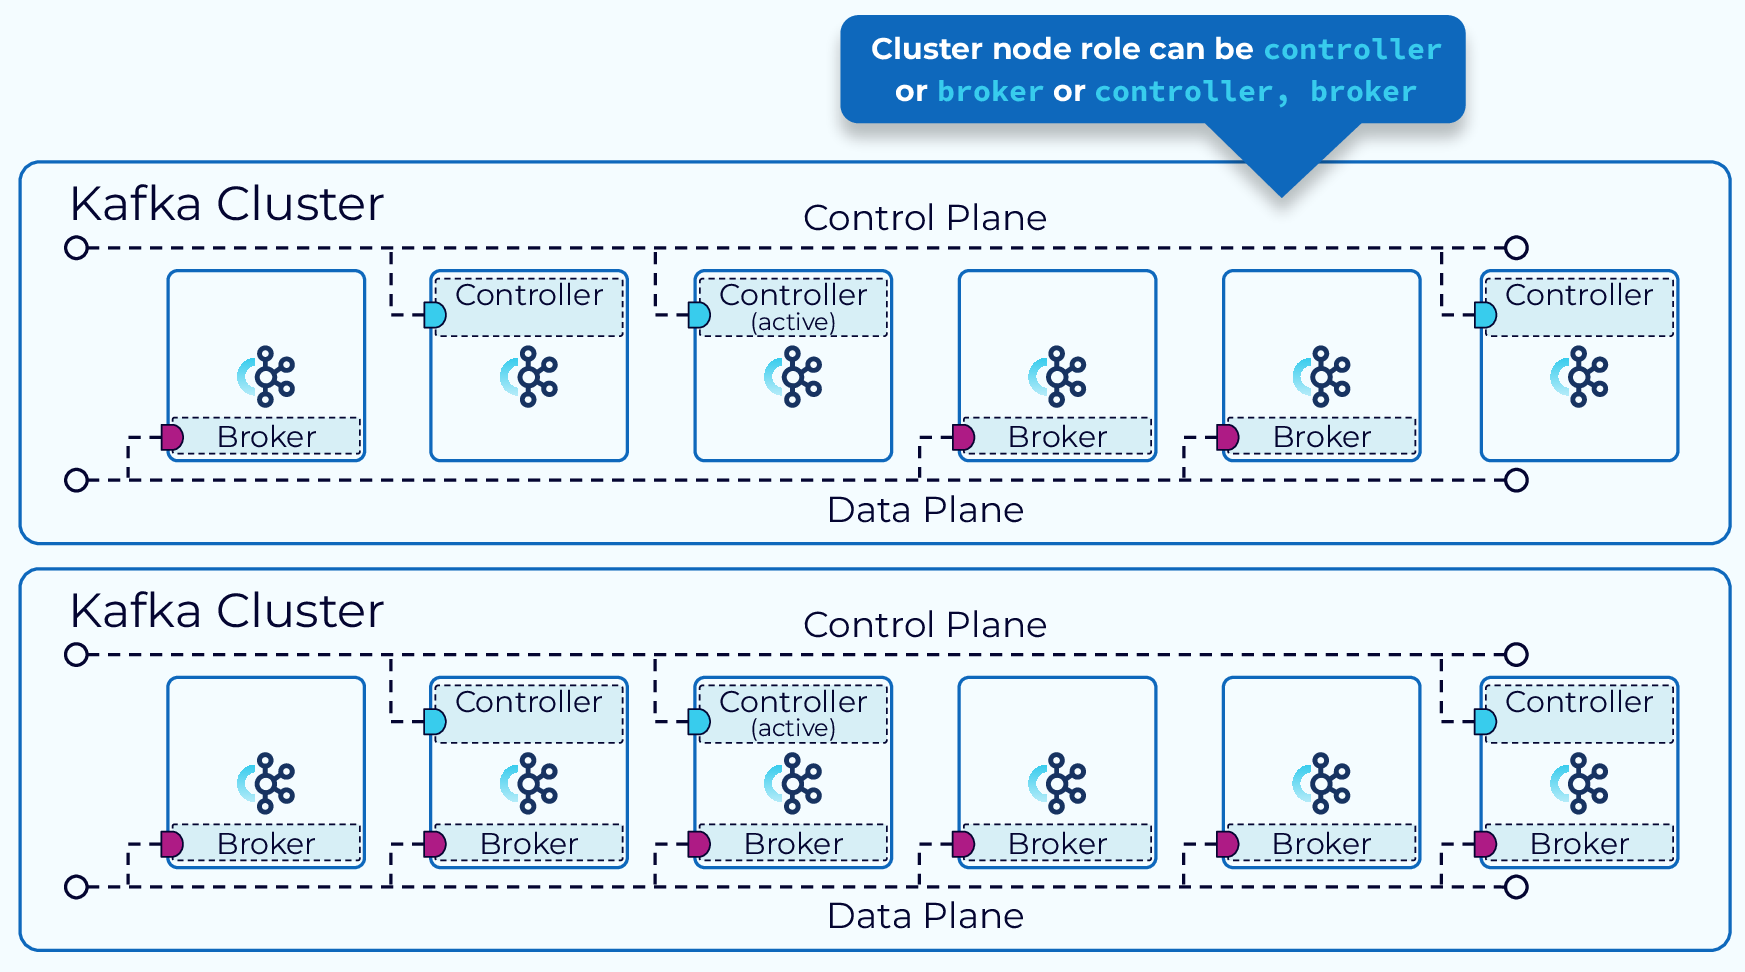
\includegraphics[width=0.75\linewidth]{figures/Kafka_Internals_052.png}
	\centering
	\caption{KRaft Cluster Node Roles. \href{https://developer.confluent.io/courses/architecture/control-plane/}{[Ref]}}
	\label{Kafka_Internals_052}
\end{figure}

Applying the correct configurations, each Kafka cluster in a multi-broker implementation becomes fault tolerant. Kafka controllers are responsible for the load balancing and the fault tolerance of any Kafka application. 
Furthermore, Kafka's ability to provide high throughput and low latency ensures that applications using it are not only fast and responsive, but also safeguarded against data losses due to run time failures. Multi broker implementations combined with the new KRaft control protocol offer faster response times whenever data recovery is needed, which usually occurs in the case that one or more brokers fail during their operation. In alignment with the Apache Kafka project's current recommendation, we have opted to use KRaft as the controller in our thesis, replacing Zookeeper, which has been deprecated for new deployments \cite{KraftRecommendation}.

\subsection{Kafka Topics}\label{kafka_topics}
Going a step further, Kafka uses topics to manage and securely store events. Topics function like folders in a file system, with events acting as the files within. New event messages are appended to the end of the topic and, once written, these events are unchangeable. In Kafka topics, unlike other messaging systems, events are not deleted post-consumption. Instead, a retention period is set, beyond which messages are deleted, with the maximum duration being up to one week. The performance of Kafka remains stable regardless of data stored, implying that long-term data storage should have a minimal performance impact.
\subsection{Kafka Partitions}\label{kafka_partitions}

\begin{figure}[htbp]
	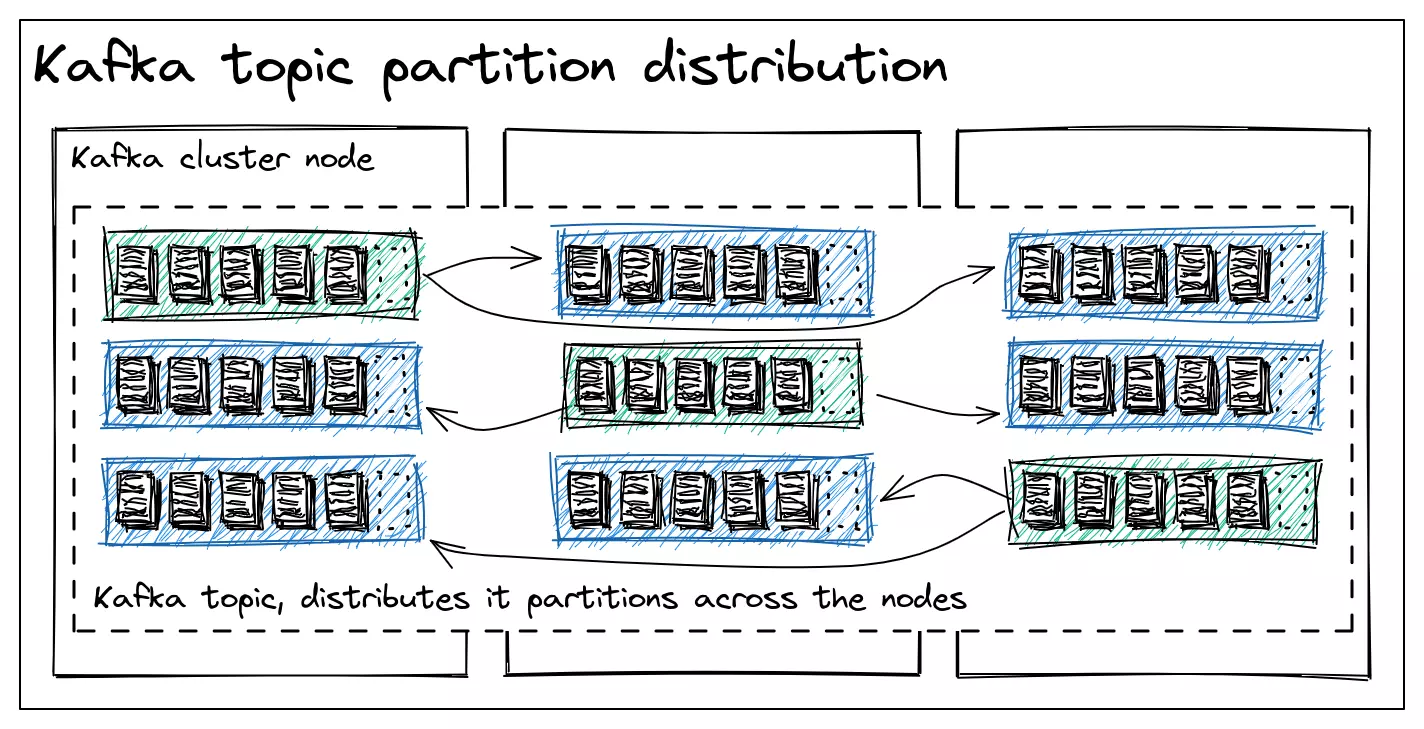
\includegraphics[width=0.75\linewidth]{figures/partition-distribution.jpg}
	\centering
	\caption{Kafka topic partition distribution. \href{https://trigodev.com/de-at/blog/kafka-topics-and-partitions}{[Ref]}}
	\label{PartitionDistribution}
\end{figure}

Kafka topics are segmented into partitions. A single topic in Kafka is divided into multiple partitions . Partitions are distributed across Kafka brokers in the cluster and messages are shared among multiple nodes. The performance of reading, writing and processing events is maximized and data is replicated across all Kafka nodes, presented in Figure \ref{PartitionDistribution}. New events are appended to a specific partition within a topic and events with the same key are stored in the same partition, ensuring data ordering. This partitioning mechanism contributes to the high throughput and fault tolerance capabilities of Kafka.

\section{Existing Event Streaming Protocol Integration}
We support different protocols currently available on the SYNAISTHISI platform. Since most IoT devices and applications primarily use the RabbitMQ and MQTT protocols, our primary focus is to interconnect these protocols with our Kafka components.
\subsection{RabbitMQ}
RabbitMQ \cite{RabbitMQ} is an open-source message broker, also known as a message-oriented middle-ware. It implements the Advanced Message Queuing Protocol (AMQP) and supports several other protocols. RabbitMQ provides robust messaging for applications. It is easy to use, runs on all major operating systems and supports a huge number of developer platforms. It also provides a wide range of features to let you trade off performance with reliability, in means of persistence, delivery acknowledgments and high availability. The key supported protocols are AMQP, MQTT, STOPMP, HTTP and Web Sockets. Additionally, it offers multi-language client support, providing a wide range of development platforms of the most popular programming languages and frameworks like Python, Java, .NET, JavaScript, Ruby, Go, etc. RabbitMQ can be deployed in distributed and federated configurations to meet high scale and availability requirements. It offers flexible routing and bridging mechanisms, along with fault tolerance features such as clustering, automatic fail-over and message durability. This wide variety of protocol support and accessible bridging between those protocols make RabbitMQ a valuable tool for the IoT market, while worldwide large-scale companies also use it, mainly for their messaging infrastructure.
\subsection{MQTT}
MQTT \cite{MQTT} stands for Message Queuing Telemetry Transport. It is a lightweight publish-subscribe network protocol capable of transporting messages. It is designed for restricted devices and low-bandwidth, high-latency, or unreliable networks. The protocol ensures reliable message delivery and minimizes network bandwidth requirements. It provides one-to-many message distribution applications and message retainment, since an MQTT topic holds the last messages and the next time a client subscribes, it immediately receives these messages. The low transport overhead and quality of service options provided by MQTT make it an ideal choice for scenarios where network bandwidth is limited and connectivity is unreliable. Thus, its lightweight nature and efficient use of network resources make MQTT a popular choice in the IoT ecosystem, where devices often operate under unstable network conditions and power limitations.

\section{Kafka Connect}
\label{kafka_connect}
Kafka Connect \cite{KafkaConnect} is a robust framework that allow us to interconnect our Kafka cluster with external systems such as databases, search indexes and different kinds of communication protocols. It is designed to handle various event streaming use-cases, including scalable and reliable streaming of data to and from Kafka. The framework is designed around a simple concept of connectors and workers. Source connectors import data from systems and propagate it to Kafka, while Sink connectors export data from Kafka to external systems. Connectors manage the integration between Kafka and other systems and they can be created without the necessity of additional code to be written. Each time we add a new external framework to our stack , we usually need to write the code that interconnects it with our Kafka cluster. Ηowever, this type of code does not provide any advantage to our application compared to other similar applications, especially in systems where a lot of services that need to communicate with each other are involved. This resolves much trouble during the development time of a specific application, as it removes the necessity of writing undifferentiated code for those external interfaces every time a new one is incorporated. All undifferentiated code interfacing with other systems is bundled into separate libraries, allowing us to deploy only the necessary connectors. Furthermore, Kafka Connect is a highly acceptable solution for interconnecting different protocols to our Kafka implementation. 

Connect uses numerous connectors, among which we utilize the RabbitMQ and MQTT source-sink connectors. This allows us to interconnect these protocols that already exist in the SYNAISTHISI platform with Kafka. If necessary, we could indeed create our own connectors, providing us with the flexibility to manage virtually any data integration requirement. Kafka Connect includes a REST API for managing and monitoring connectors through workers. This API allows us to deploy, remove, pause, resume and check the status of workers associated with their corresponding connector. Automatic offset management is provided, therefore in case a connector fails, the replacement can resume exactly where the previous one stopped, guaranteeing data consistency. Kafka Connect is a powerful tool that simplifies the process of integrating different systems with Kafka and empowers robust, scalable and reliable data pipelines in our implementation. 

\section{Schema Registry}
Kafka Schema Registry \cite{SchemaRegistry} offers a REST interface for storing and retrieving schema registries and is an essential part of the Apache Kafka ecosystem. Its role is crucial in maintaining the consistency and well-defined nature of the data in Kafka topics. Kafka Schema Registry is used in combination with Apache Avro \cite{Avro}, providing a data serialization system that encodes data in a compact binary format . Avro schemas define the structure of the data being encoded, making it easy for each consumer to correctly deserialize the data. This advanced and compact binary format allows us to significantly reduce the event’s message size, especially in instances where the producer is utilizing the JSON format.


\begin{figure}[htbp]
	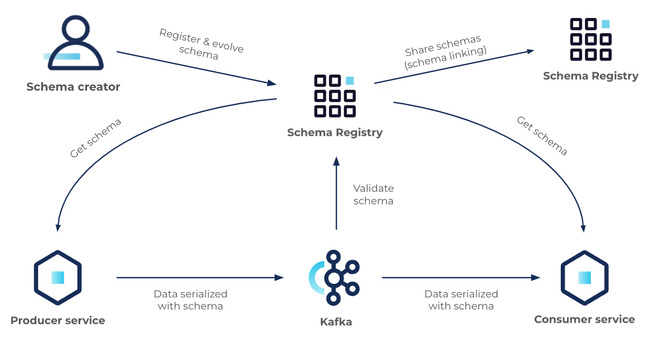
\includegraphics[width=0.75\linewidth]{figures/schema-registry-ecosystem.jpg}
	\centering
	\caption{Schema Registry architecture overview \href{https://docs.confluent.io/platform/current/schema-registry/index.html}{[Ref]}}
	\label{SchemaRegistryEcosystem}
\end{figure}

The primary purpose of a schema registry, is storing and retrieving schemas in a centralized location, presented in Figure \ref{SchemaRegistryEcosystem}. Producers and consumers that utilize schema registry, own a contract of what type of data to expect, reducing the possibility of data inconsistency and parsing errors . Schema evolution is supported to accommodate the inevitable changes in our data over time, reflecting the evolving needs of our applications. This ensures our system remains flexible and adaptable to meet these ongoing changes. The support for schema versioning in our system allows us to maintain compatibility with older data that was encoded using previous versions of the schema, providing seamless access and utilization of older data structures. 

In summary, Schema Registry is a crucial tool for maintaining compatibility and data integrity in Kafka-based systems. It provides a centralized store for schemas, supports schema versioning and evolution and allows for a clear contract between producers and consumers. Over the past few years, it has emerged as an industry standard for event streaming applications, driven by the increasing need for data size reduction and compatibility in the face of growing data volumes and complex processing requirements.
    \chapter{Architecture and Implementation}
\label{chap4}
In this chapter, we are going to analyze and present the technical details of our project. 
We explore the critical aspects of our project, focusing on the implementation and execution of our designed solution. In addition, we provide details on the system's architecture, the chosen configurations and a further explanation of the key fundamentals that were prioritized for our implementation. Furthermore, we outline the main challenges encountered during the implementation phase and how we addressed them.

\section{System Overview}
\label{system_overview}
Our system is divided into three primary layers: the data ingestion processes, the events streaming and storage and data consumption and distribution in our front-end map. The system's architecture is presented extensively in Figure \ref{SystemArchitecture}.

Starting from the top, three protocols for producers are supported: native Kafka, AMQP and MQTT. A RabbitMQ broker within the SYNAISTHISI platform manages messages generated by MQTT and AMQP clients. Subsequently, Kafka Connect interlinks our events from the RabbitMQ broker with our Kafka Cluster. We primarily utilize source connectors for our air quality application, meeting our data flow requirements. The Schema Registry is mainly used for our native Kafka producers, in order to validate our data and minimize the message size sent to our Kafka cluster. Avro is utilized as the serialization format in our Schema Registry service.

Events are subsequently streamed into our Kafka cluster. Our cluster operates in KRaft mode and consists of four nodes. A single controller node maintains the health of our Kafka cluster and performs tasks related to load-balancing and data recovery, in the cases that runtime failures occur. The remaining three nodes are data brokers configured in prioritizing data reliability, availability and ordering. In order to monitor and manage our Kafka Cluster and its associated services, such as Kafka Connect and Schema Registry, we have integrated an advanced control panel. AKHQ \cite{AKHQ} provides us with a user friendly graphical interface, allowing us to maximize our operational capabilities in a modern and accessible manner.

\begin{figure}[htbp]
	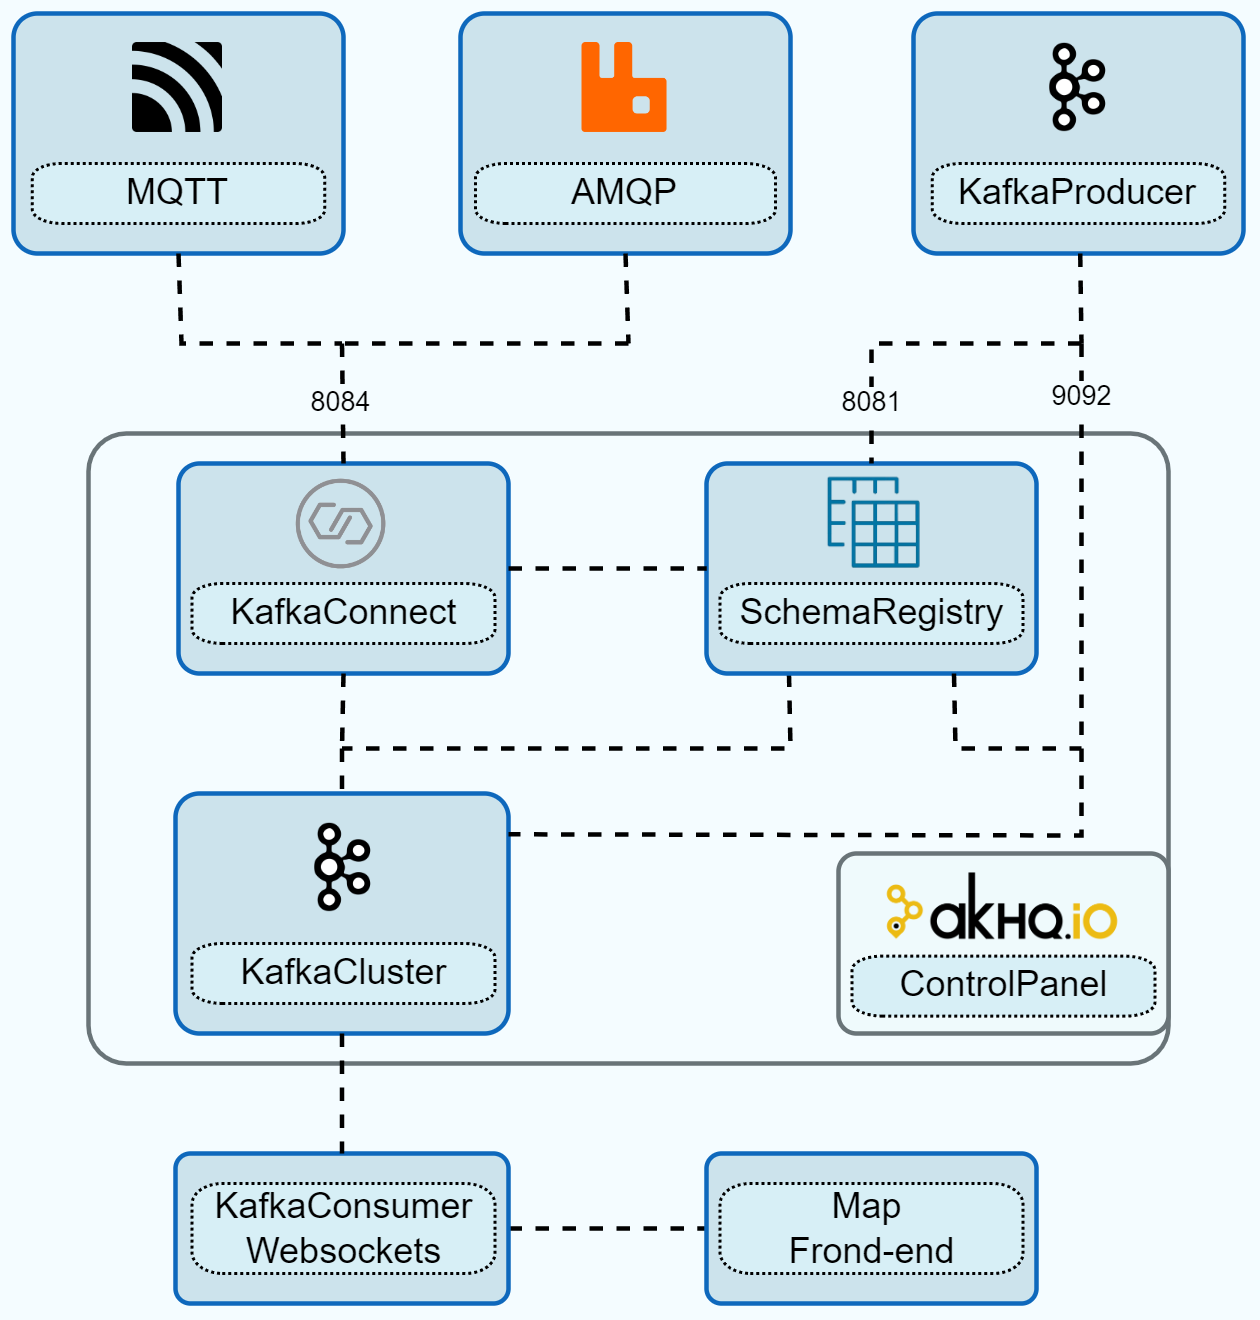
\includegraphics[width=0.75\linewidth]{figures/scheme.drawio.png}
	\centering
	\caption{System Architecture}
	\label{SystemArchitecture}
\end{figure}

Additionally, a web application has been developed to display measurements on a live map. An automated process parses through the Kafka topics and assigns consumers to them. Both simple and Avro consumers are orchestrated to work in sync to fetch live events from our cluster. Web-Sockets, over a TCP connection, is continuously active application, ready to transfer data from our server side to our web browser. For our front-end we utilize React \cite{React} and OpenStreetMap \cite{Openstreetmap} to present the measurements on a contemporary, visually appealing map-based web page. Each point on the map represents sensors that continuously update and refresh their values. This configuration guarantees real-time and precise data representation, while ensuring low latency, high throughput and optimal availability.


\section{Data Ingestion}
Continuing with the principles of the SYNAISTHISI platform, we provide support for the primary messaging protocols that are found in the majority of IoT infrastructures. This support allows us to establish connections with a wide variety of sensors, gateways and devices. By doing so, we enable the interoperability, scalability and interconnectivity principles that our application requires. Aside from our focus on air pollution measurements, our platform is capable of utilizing any type of data that is supported by these protocols. This flexibility helps us to adapt and configure our application for different kinds of implementations. Furthermore, we are not only confined to the typical messaging protocols that are commonly used in IoT applications, but utilizing more advanced protocols like Avro. Avro allows us to handle more complex data structures and provides us with additional capabilities, enhancing the overall functionality, versatility and upgradability of our platform.

\subsection{Producers}
We have created a set of producers for each protocol, aiming to simulate the respective clients that would publish our measurements to our brokers. These producers are written in Python in our implementation, but the operators of our application can choose any language pack depending on the compatibility of their devices and gateways. Our primary messages are based on the JSON file format, that provide us a broad system support and the ability to configure the rest of our infrastructure based on an internet standard message type. The majority of messaging and event-driven applications primarily use JSON due to its simplicity and widespread support across virtually all cloud infrastructures.

\label{producers}
Additionally, messages are structured in JSON files containing the following fields: DeviceID, Latitude, Longitude, PM\textsubscript{2.5} concentration in micro grams per cubic meter of air (\si{\micro\gram\per\/\cubic\meter}), Humidity in percentage (\%), Temperature in Celsius (\si{\celsius}) and Timestamp, as can be seen in Figure \ref{json_avro}. DeviceID is the name or label of a given device that fetches measurements. Latitude and longitude represent the coordinates where each device is located and enable us to locate our device on our live map. If our devices support GPS, the coordinates should be imported to these fields, otherwise operators should input the approximate location. PM2.5, temperature and humidity are the primary data needed for our air quality application. The Timestamp field provides us with the time and date when our event took place.

\subsection{Interoperability Kafka Connect }
The data produced by MQTT or AMQP clients, are directed to our SYNAISTHISI RabbitMQ server. In this manner, we have implemented Kafka Connect to fetch our data from our RabbitMQ broker to our Kafka cluster. We have integrated both source and sink connectors for MQTT and AMQP, therefore supporting bidirectional communication between RabbitMQ and Kafka. In our application, we utilize the source connector (which inserts data from an external system into our Kafka Cluster) for both MQTT and AMQP, as it aligns with our application's data flow requirements. This setup enables our Kafka infrastructure to interact with external systems in a straightforward and accessible manner.

Connectors are configured in distributed mode, which allows us to replicate the deployed workers, activating the fault-tolerant capabilities of Kafka Connect workers. It is worth noting that we deploy a single worker on each connector, not multiple ones, but users of our platform have the option to replicate the workers in case they want to protect the Connect workers from runtime failures. Our workers can be both schema enable or not, enabling the data validation routine for non Kafka producers as well.
As discussed in Kafka Connect section (cf. Sec. \hyperref[kafka_connect]{3.4}), Kafka Connect allows us to interconnect our Kafka cluster with a wide variety of external systems and services. This eliminates the need to write additional code each time we integrate a new external service, thus significantly reducing our development time.

\subsection{Data Validation Schema Registry}
We also utilize the Schema Registry in our application, both for native Kafka producers and for Connect workers. Schema Registry allows us to implement a more compact communication protocol. The initial JSON messages are serialized into an efficient binary format, ready to be broadcast to the Kafka Cluster. This process enables us to reduce the size of the JSON events that are sent to our Kafka Cluster, decreasing the message size by 40\% or more, depending on the size of the JSON files and the number of fields. The more fields a JSON file has, the greater the reduction in message size, thanks to the efficient compression in Avro. It requires the initial message to be in JSON format before being converted, ensuring a consistent event data structure whether we utilize the Schema Registry or not. One advantage of Avro over similar protocols is its wide support across various communication and messaging infrastructures. This makes our platform highly efficient, sophisticated and highly configurable, depending on our implementation

In our implementation, our Kafka producers utilize Avro. This gives us comprehensive control over our data structure and the fields necessitated in our JSON files. We generate an AVSC file, which is a JSON format file that defines the schema or structure of the data to be serialized using Avro, as shown in Figure \ref{json_avro}. For instance, if we desired to make the 'Humidity' field optional and the 'PM\textsubscript{2.5}' required, the message streaming would persist even if the former missing, but would stop if the latter was missing. In our implementation all fields are required, so we designate them all as mandatory. This provides a centralized way to supervise and monitor our data structure and compatibility in an organized and secure manner. Last but not least, data sent from our MQTT and AMQP connectors in our air quality application do not utilize the Schema Registry, as we want to simulate situations where we interconnect our platform to pre-existing sensors and aim to avoid developing new code when connecting them.

\begin{figure}[htbp]
\begin{minipage}[t]{0.4\textwidth}
\begin{lstlisting}
  "deviceId": "sensor2",
  "latitude": 39.36103,
  "longitude": 22.94248,
  "pm25": 12.5,
  "temperature": 22.5,
  "humidity": 60.0,
  "timestamp": 164099520
\end{lstlisting}
\end{minipage}%
\hfill
\begin{minipage}[t]{0.55\textwidth}
\begin{lstlisting}
"type": "record",
"name": "SensorData",
"fields": [
{"name": "deviceId", "type": "string"},
{"name": "latitude", "type": "double"},
{"name": "longitude", "type": "double"},
{"name": "pm25", "type": "float"},
{"name": "temperature", "type": "float"},
{"name": "humidity", "type": "float"},
{"name": "timestamp", "type": "long"}]
\end{lstlisting}
\end{minipage}
\centering
\caption{Presentation of our JSON file (on the left) and our Avro Schema (AVSC, on the right).}
\label{json_avro}
\end{figure}

\subsection{Data Structure}
\label{data_structure}
In the Events and Producers sections (see Sec. \hyperref[events]{3.2.2}, \hyperref[producers]{4.2.1}), we discuss how our JSON messages are structured in both a general event message example and in our specific implementation. However, the format presented is the human-readable one, which is how the data will appear on our front-end page. The actual JSON files, when ingested into our Kafka cluster, will appear as shown in Figure \ref{json_avro}. Most of the fields remain understandable and human-readable, even in this form. The exception is the timestamp, as we utilize Unix epoch time, which represents a specific time as a single number. The Unix timestamp is widely adopted in most computing environments due to its compact size and simplicity for data storage and transmission. Therefore, we only need to convert it into a human-readable form when we intend to display it in our application, while our data structure remains highly scalable and flexible.


\section{Kafka Cluster Configuration and Management}
During the development of our Kafka Cluster, we faced a series of challenges. Our primary objective was to create a platform that would be highly available and easily upgradable for integration with other applications too. The configuration we chose for our Cluster reflects that of a production environment, minimizing the need for operators to make further extensive configurations when hosting their own applications on this part of our platform.
We designed an implementation that aligns closely with enterprise-level features and requirements, while maintaining IoT principles of simplicity and ease of use. 

Our implementation is developed to seamlessly interconnect with our existing SYNAISTHISI platform , ensuring a unified and interconnected system. We leveraged the latest technologies to optimize our Cluster's performance, achieving high-speed data streaming and processing without compromising its robust fault tolerance capabilities. This balance between speed and reliability is a critical aspect of our project, as it ensures our platform can handle large volumes of data while maintaining durability during runtime failures. By addressing these challenges, we have created a Kafka Cluster that is not only powerful, scalable and reliable but also adaptable and user-friendly, making it a valuable tool for anyone who wishes to take advantage of it.

\subsection{Cluster Configuration}

Our cluster is structured in a four-node Kafka implementation, as depicted in Figure \ref{ClusterConfiguration}. Our nodes function either as controllers or data brokers, with a single node and three nodes serving as the controller and data brokers respectively. This is the recommended production implementation by the Apache project, as combined controller/broker nodes are primarily used for presentations, early development and testing purposes. This setup allows us to leverage the high throughput and fault tolerance features that Kafka is capable of. Furthermore, depending on the demand of our application, we have the flexibility to scale our cluster from three brokers to five, seven and beyond. This scalability ensures that we can meet the increasing demands, if needed, without compromising the performance or reliability of our system.
 
Instead of opting for the deprecated Zookeeper control plane, we employ the relatively new KRaft protocol. Adopting KRaft significantly increases the speed of data recovery and re-balance time when a broker node fails during operation and it provides better metadata management compared to Zookeeper. The internal configuration we have established allows us to expose only a single port (9092) of our cluster. The rest of the data flow is contained within our cluster, eliminating the need to expose our system further. This approach enhances the security of our implementation while maintaining its efficiency and effectiveness, as shown in Figure \ref{SystemArchitecture}.

\subsection{Control Plane}

Furthermore, we utilize a single controller node in our control plane without replicating it, as seen in Figure \ref{ClusterConfiguration}. This approach helps us avoid unnecessary complexity and overhead, without direct exposure to the risk of data loss. We need to note that this decision was made after careful consideration of our requirements and priorities. While replicating the controller node could theoretically increase fault tolerance, it would also introduce complexities and potential synchronization issues. Instead, our focus on fault tolerance is achieved through replicating only the data brokers. This way, even if our controller node goes down during runtime, our data within the brokers remains safe. By leveraging a single node control plane configuration we achieve a firm balance between simplicity and robustness in our Kafka implementation.

\begin{figure}[htbp]
	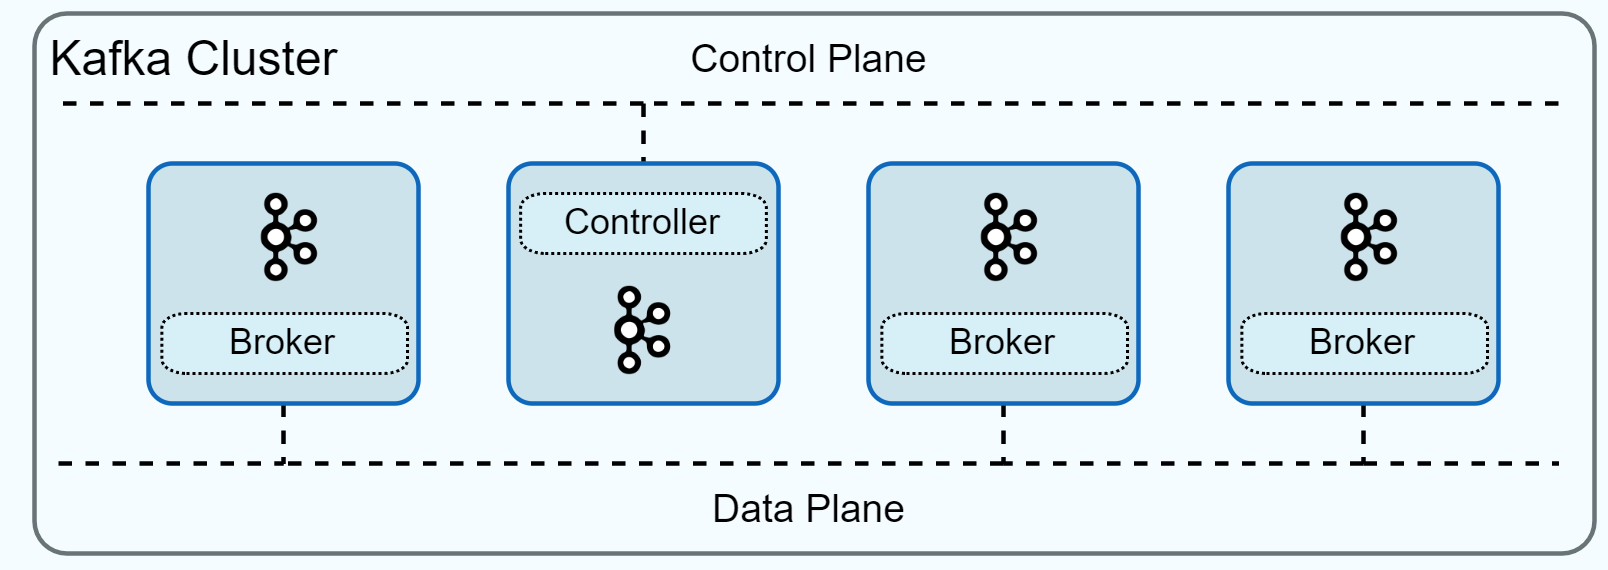
\includegraphics[width=0.75\linewidth]{figures/cluster.drawio.png}
	\centering
	\caption{Cluster Configuration}
	\label{ClusterConfiguration}
\end{figure}

\subsection{Data Plane}
Our three broker data plane endows our system with enhanced reliability, fault tolerance and scalability. Firstly, this configuration offers superior fault tolerance compared to single and two-broker clusters. In the event that one of our brokers fail, Kafka will redistribute the load across the remaining two brokers. Since we are utilizing KRaft, the time needed for our Kafka Cluster to re-balance the replicated data is significantly minimized. The residual two nodes are able maintain the data flow, ensuring minimal downtime during our cluster and application operation. This approach guarantees high availability for our platform, preventing disruption to our data streaming process in case of a broker failure.

Moreover, in terms of scalability, a three broker configuration is beneficial as the workload is distributed across multiple nodes. This arrangement distributes our data across each broker, ensuring a balanced workload. If the data volume and processing requirements escalate, we can increase the partition count on any given topic. Given the design of our data plane, we have the flexibility to easily expand our infrastructure with additional brokers if necessary. This ability to scale horizontally allows us to adjust to changing workload demands and ensures our platform is prepared for future expansion and enhancements. In this way, we have achieved an optimal balance between fault tolerance and scalability, making our implementation adaptable to a broad range of use cases.

\subsection{Control Panel}
Last but not least, we have implemented a control panel using AKHQ, which provides a contemporary and accessible graphical interface for managing our Kafka Cluster and its associated services. In addition to the SYNAISTHISI platform interface, operators can utilize this control panel to create topics, seen in Figure \ref{ControlPanel}. It also facilitates schema creation, modification and evolution within our Schema Registry service. All Kafka Connect workers can be deployed and controlled from this panel, simplifying monitoring and management during application runtime. This eliminates the need for users to rely on CLI (Command-line interface) tools, offering a more modern management method. As both self-managed and fully-managed cloud service providers rely on graphical interface control panels for their operations, our approach aligns with this standard. AKHQ is based on an open-source project with numerous contributors, guaranteeing its ongoing support and maintenance.

\begin{figure}
    \centering
    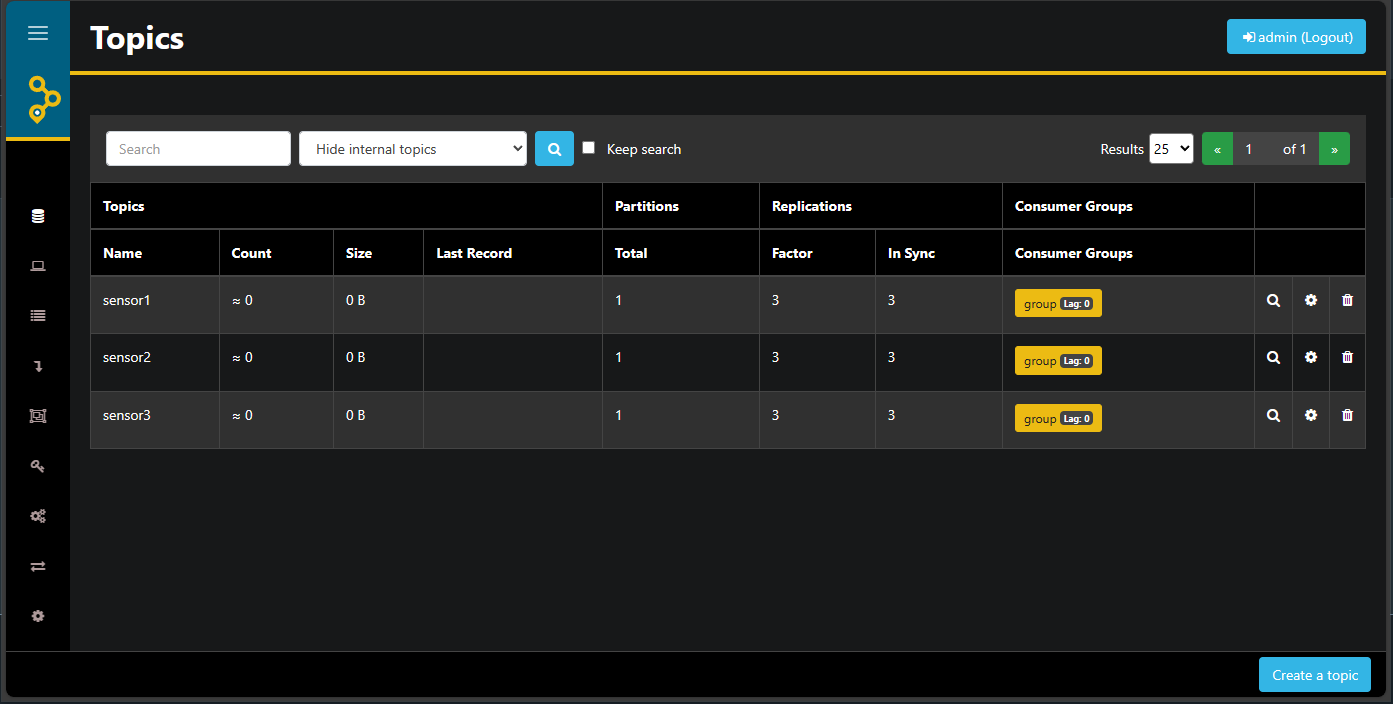
\includegraphics[width=1\linewidth]{Screenshot 2024-01-25 141106.png}
    \caption{Control Panel Overview}
    \label{ControlPanel}
\end{figure}

\section{Web Application}
In this section, we analyze the creation of a server-less side, back-end service and front-end page. These components fetch data from our cluster and display them on a live map. This implementation is specifically designed for our air quality application and is not a general-purpose platform like the Data Ingestion and server-side parts. On this regard, we have implemented a service that consumes live data from our Kafka Cluster and automatically detects the addition of new devices in our cluster. The consumed events are then sent over Web-Sockets to our front-end map, which is hosted as part of our modern-looking React live page.


\subsection{Kafka Consumer}
Whenever a topic is added to our server-side, the back-end service automatically detects the newly added topic. Each sensor, device, etc. on our map is uniquely identified by the key that has been assigned to it. Kafka consumers then read the incoming live events and list them in a batch of messages. In our application, the consumption rate is every five minutes, but this can be modified to any preferred frequency. Consumers can either be simple Kafka consumers or schema-enabled ones, as our universal JSON event message structure allows us to utilize both without any incompatibilities. This highlights the importance of having a firm and well-thought-out structure for our event streaming data, as it allows us to consume and process our events efficiently, eliminating the time required for post-consumption data modifications from the cluster.


\subsection{Web-sockets Integration}
To facilitate the interconnection between our back-end service and front-end map, we utilize Web-Sockets. Web-Sockets is a protocol that unlike traditional HTTP connections, establishes a continuous communication channel over a single TCP connection between the front-end and back-end. Web-Sockets does not have any limit on the batch size that can be transmitted, making it an excellent choice for our needs of continuous data flow for the events consumed by our Kafka Consumer service. This ensures flawless real-time data transmission and enhances the responsiveness of our application. Furthermore, we minimize the need for frequent HTTP polling, which enhances our application's network efficiency. Therefore, by leveraging Web-Sockets, we can effectively align with the high-volume and real-time data streaming capabilities that our Kafka infrastructure is offers.

\subsection{Front-end Map}
Our live front-end map is developed utilizing React, a modern and efficient development environment. This framework allows us to create a visually appealing and highly functional web page, ideal for displaying real-time data. The map we utilize is based on Leaflet OpenStreetMap, an wide spread open-source map solution that perfectly suits our application needs. In addition to its efficiency, The component-based architecture of React enables us to easily manage and update our application's interface, ensuring a smooth user experience.

Our web page is divided into two primary sections, the map section and the data section. In the map section, Figure \ref{ReactMap1},each point represents a sensor at a specific location. When a point is selected, it displays the measurements from the corresponding sensor. As detailed in the Data Structure section (cf. Sec. \hyperref[data_structure]{4.2.4}), our measurements include the device name, the time of the measurement, PM\textsubscript{2.5} concentration (\si{\micro\gram\per\/\cubic\meter}), Humidity (\%), Temperature (\si{\celsius}). The data is presented in a bracket when each point on the map is selected. Whenever a new device is incorporated into our platform, a new point is automatically created on the map according to the device's coordinates. Consequently, this way our map page maintains a dynamic, user-friendly and modern design.

The other section of our page features a set of dashboards, Figure \ref{ReactMap2}, each designed to display the three key measurements from our sensors: particle matter concentration, humidity percentage and temperature. Each set of tables within the dashboards corresponds to a specific point on the map. As these points are dynamically updated on the map to reflect the real-time locations of our sensors, the relevant tables in the dashboards adjust accordingly. This ensures that the set of data displayed is always updated. Moreover, the system allows us to display measurements from various time frames. Users can view measurements from a single day, three days, or a week old, providing them a comprehensive view of understanding of fluctuations over these periods over these periods.

\begin{figure}[htbp]
    \centering
    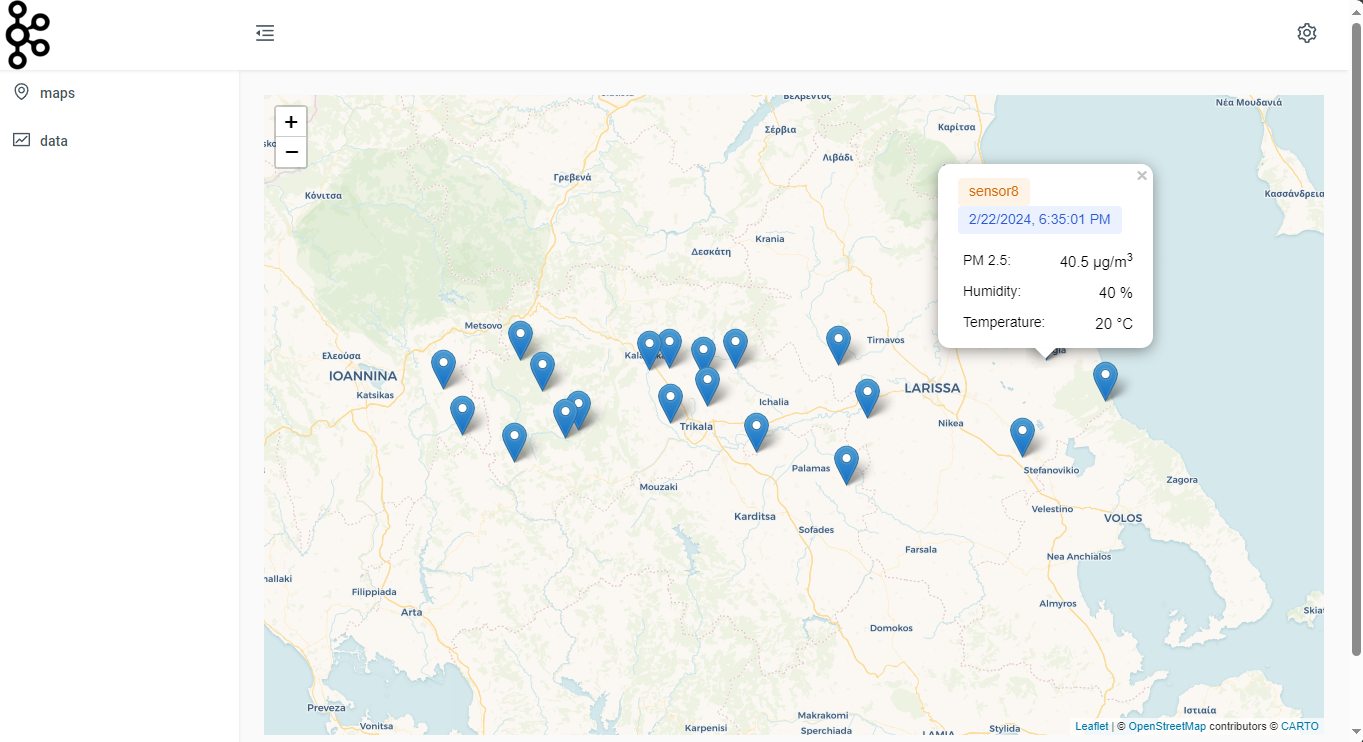
\includegraphics[width=1\linewidth]{figures/Screenshot 2024-02-22 183525.png}
    \caption{Live Map Overview}
    \label{ReactMap1}
    
    \vspace{2.5cm} % Adjust the space as needed
    
    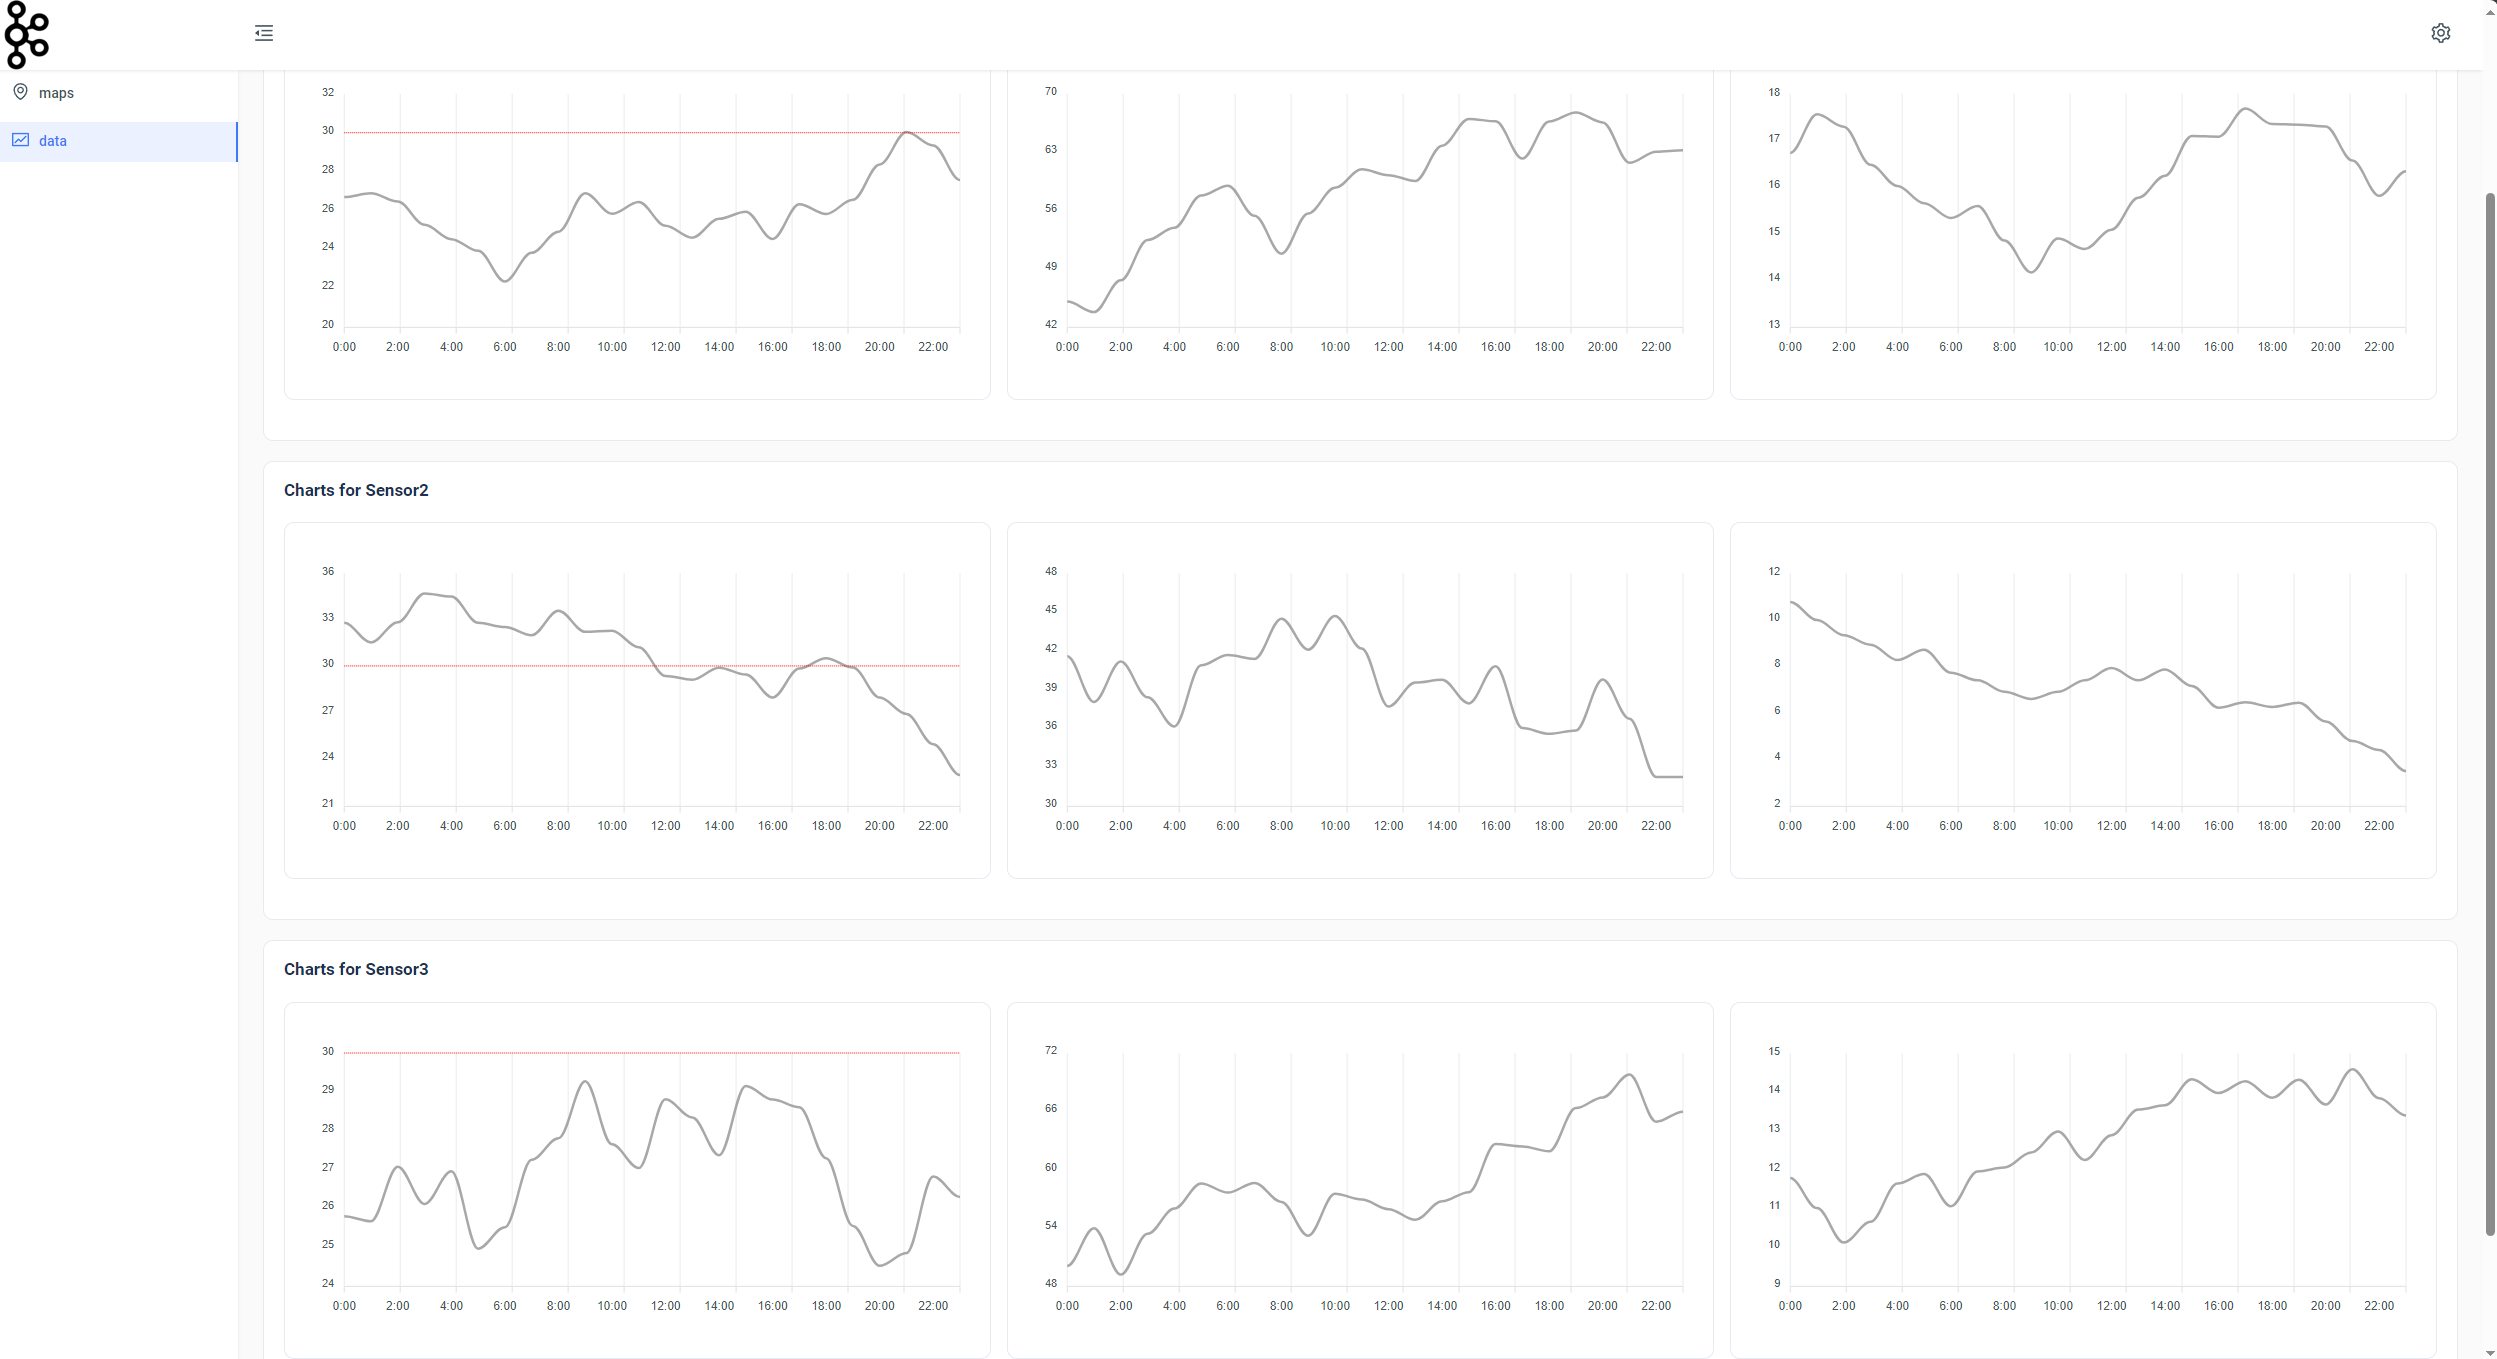
\includegraphics[width=1\linewidth]{figures/Screenshot 2024-02-22 183833.png}
    \caption{Historical Data Dashboard Overview}
    \label{ReactMap2}
\end{figure}
    \chapter{Experimental Evaluation}
\label{chap5}

At this point, we have described our primary motivation and background, and comprehensively analyzed the architecture and implementation of our application. In this section, we execute a series of realistic routines to demonstrate the key principles of our implementation. We test the data validation process and message size reduction. Finally, we deploy a realistic number of producer clients, generating data for our Kafka cluster, so that we can evaluate its throughput. 
%Finally, we employ AMQP and MQTT clients to determine whether there is a significant delay difference between native Kafka producers and Connect ones.

\section{Data Validation Routine}

In order to test our data validation routine we have prepared a set of scenarios, configuring our schema, Figure \ref{json_avro}, depending on the use cases and our needs.

\begin{enumerate}
    \item Firstly, we can configure all fields in our schema, to default to null values. This allows for normal event parsing to our Kafka Cluster even if any fields in our JSON input file are missing. While this configuration offers maximum flexibility, it does not check our data before it is published to our application.
    \item In the second scenario, we select a few or just one value to default to null. For instance, we could set our temperature field to null in our schema if a group of sensors or devices doesn't support this measurement. In this instance, messages would still be parsed even if the temperature field was missing from the input messages.
    \item The third scenario involves not setting any field to default at null. This enforces strict data validation, requiring all our fields to be included in our input file.
    \item The fourth case involves disallowing additional fields beyond those included in the schema fields. By default, the schema registry permits extra fields if the required ones have been validated. For example, if an incoming message includes an additional 'pressure' field, we can decide whether or not we want this event to be produced.
\end{enumerate}

In the four scenarios outlined, our goal was to showcase the versatility of our schema registry implementation. As a result, we ranged from a highly flexible data validation routine to a very strict one. The degree of flexibility is dependent on the requirements of our application and implementation at each instance. This underscores the importance of maintaining a balance between adaptability of data and its consistency.

\definecolor{color1}{RGB}{133,147,148}
\definecolor{color2}{RGB}{29,52,94}


\section{Event Size Reduction}

\begin{table}[htbp]
\centering
\begin{tikzpicture}[trim axis left, trim axis right]
\begin{axis}[
    ybar,
    bar width=0.9cm,
    width=0.8\textwidth,
    height=0.5\textwidth,
    ylabel={MegaBytes},
    symbolic x coords={7.000, 70.000, 700.000},
    xtick=data,
    ymin=0,
    ymax=150,
    enlarge x limits=0.37,
    ymajorgrids = true,
    grid style={dashed}
    ]
\addplot[fill=color1] coordinates {(7.000, 1.402) (70.000, 14.02) (700.000, 140.19)};
\addplot[fill=color2] coordinates {(7.000, 0.707) (70.000, 7.076) (700.000, 70.76)};
\end{axis}
\end{tikzpicture}
\caption{JSON to Avro size of messages comparison }
\label{avro_vs_json}
\end{table}
Our Schema Registry implementation enables us to store events in our cluster in a more compact and efficient manner. We produced a set of messages to observe the size reduction between native or string JSON format messages, and Avro serialized ones. Our data sets are in groups of 7,000, 70,000, and 700,000. As presented in table \ref{avro_vs_json}, the size reduction ranges from 1,402 KB to 707 KB, 14.02 MB to 7.076 MB, and 140.19 MB to 70.76 MB, for the batched 7,000, 70,000 and 700,000 messages respectively. Therefore, the reduction rate for our input message when converted to Avro format is $\approx$ 48-50\%. This size reduction can vary based on the structure of the original fields and the initial event size, and it can be increased even further. Although the size reduction in our case is in the range of megabytes, it is clear that this sets the stage for larger scale implementations where tens or even hundreds of millions of events are constantly stored in the clusters.



\section{Throughput Testing}

We have created a realistic deployment scenario to test whether our implementation can handle the expected payload. In this scenario, we emulate a situation with a hundred devices producing data, setting up a hundred producers that constantly send data to our Kafka cluster. However, in our tests, we produce messages every second and every five minutes. This dual frequency approach provides a clear view of the volume of messages our implementation can handle, both with our standard deployment frequency, and with a significantly higher one.
Often, benchmarks test throughput in unrealistic environments. By conducting realistic tests, we can confirm that our implementation can handle the load during production. We leverage Kafka's partition mechanism in this process, with each of the hundred devices representing a hundred partitions. This is an optimal use case where each partition is connected to a single device.

Given that our production message frequency is every five minutes, by sending messages every second in our cluster, we emulate the behaviour of having a significantly larger number of devices publishing messages. It is also important to note that throughput results often depend on the event message size. 
Therefore, we conduct our experiment using our application's message structure. The experimentation was carried out on an i7-6700k system, utilizing Docker engine hosted on WSL2, with an allocation of 6 logical cores. Our implementation was able to handle incoming messages at frequencies of both every second and every five minutes without any downtime. Similarly, our consumer was able to read data without any downtime, even during the test with a frequency of every second. As a result, we have verified that our cluster implementation can handle a hundred messages being sent every second from a hundred different devices, based on our given system configuration.
    \chapter{Conclusions}
\label{chap6}
In this thesis, we developed a full-stack air pollution monitoring system adhering to IoT fundamentals, but also combined with capabilities found in enterprise cloud services. Our key goals and challenges were to extend the capabilities of the SYNAISTHISI platform with advanced event streaming services, create a live environmental air quality monitoring application and make our platform as scalable and interconnected as possible to host other similar applications.

We analyzed our motivations, considering the need to create air pollution monitoring applications and infrastructures accessible to the public. We created an event-driven middle-ware capable of interconnecting with most of the established protocols in the IoT industry. We configured our Kafka cluster in a containerized, multi-broker implementation and adopted the latest control plane KRaft, for managing our Kafka nodes. Furthermore, we interconnected our primary cluster with Kafka Connect and its external communication protocols like AMQP and MQTT, showcasing that almost any other supported external system, service, or database can be connected as well. We added a Schema Registry to our data flow, making our application schema-enabled and providing us with features of advanced data validation, integrity and controlled data evolution. We developed a back-end service that fetches our data from our Kafka Cluster in real-time, eliminating the need for an additional database for our live event messages streaming. We facilitated a Web-Sockets application over a TCP channel, to parse the consumed data to our front-end map, efficiently matching the high throughput requirements of our platform. Last but not least, we created a React-based live map utilizing Leaflet maps, where each device and sensor is automatically added as a point on the map. Each sensor is updated on our live map and a dashboard of tables for each corresponding sensor provides us with historical measurements for up to a week.

By utilizing and orchestrating so many different services, we focused on making them as independent and modular as possible. This way, our application remains highly scalable, accessible and configurable. The whole stack is constructed and presented in a way that showcases each layer, highlighting the re-usability and adoption of our platform in other respective projects. Additionally, each individual service was chosen with the aspect of belonging to an open-source project that is being maintained, further future-proofing our platform. Features such as fault tolerance, data validation, high throughput and data integrity, which are typically found in paid enterprise cloud solutions, were incorporated into our platform. This was achieved by carefully selecting the appropriate open-source projects and services and then optimizing and configuring them to meet our requirements. Therefore, we developed a platform that is accessible to everyone and aligns with the key IoT and open-source principles, while at the same time incorporating advanced cloud features and fundamentals.

\section{Future work}

Regarding future work, there are several improvements and upgrades that could be applied to our implementation. Initially the development of enterprise-level security by utilizing SASL\_SSL and TLS(SSL) security protocols. Our configuration would involve using SSL for internal listeners(clients) and inter-broker communications. Additionally, external listeners(clients) could be configured to utilize SASL\_SSL, integrated with a Kerberos server through the GSSAPI authentication mechanism. Such integration necessitates thorough research and testing based on the cluster's needs and priorities, in order to achieve the optimal balance between security and performance. Additionally, we can enhance the default behavior of Kafka's key mapping mechanism. This could be achieved by integrating an external load balancing service or by developing and configuring our own key hashing mechanism, to distribute the events across the partitions equally and efficiently. 
%
%%%%%%%%%%%%%%%%%%%%%%%%%%%%%%%%%%%%%%%%%%%%%%%%%%%%


%\backmatter % μην ενεργοποιείτε την εντολή
% Βιβλιογραφία - Αναφορές
	\bibliography{references}


%%%%%%%%%%%%%%%%%%%%%%%%%%%%%%%%%%%%%%%%%%%%%%%%%%%%%
% %% APPENDICES (optional) / ΠΑΡΑΡΤΗΜΑΤΑ (ΠΡΟΑΙΡΕΤΙΚΑ)
% %%

% % Εάν υπάρχουν περισσότερα από ένα Παραρτήματα
% % είναι ενεργή η ακόλουθη εντολή
% % και ανενεργή για μεμονωμένο Παράρτημα
%     % Να μην τροποποποιηθεί

\cleardoublepage\thispagestyle{plain}
~\vfill
\ifgrthesisoption
    \centerline{\huge\bf ΠΑΡΑΡΤΗΜΑΤΑ}\phantomsection
    \addcontentsline{toc}{chapter}{ΠΑΡΑΡΤΗΜΑΤΑ}
\else
    \centerline{\huge\bf APPENDICES}\phantomsection
    \addcontentsline{toc}{chapter}{APPENDICES}
\fi
\vfill

% % Μην τροποποιήσετε τις ακόλουθες εντολές
% \ifgrthesisoption
%     \renewcommand{\chaptername}{Παράρτημα}
% \else
%     \renewcommand{\chaptername}{Appendix}
% \fi

% % Πριν το κάθε Παράρτημα (για περισσότερα από ένα), 
% % ρυθμίζεται η κατάλληλη αλφαβητική αρίθμηση
%     \renewcommand{\thechapter}{A} 
%   	% Παράρτημα A

\chapter{Τίτλος Παραρτήματος \label{appendixA}}



Τα παραρτήματα περιλαμβάνουν συνοδευτικό, υποστηρικτικό υλικό (πίνακες, φωτογραφίες, ερωτηματολόγια, στατιστικά στοιχεία, αποδείξεις, περιγραφές  λογισμικών  προγραμμάτων,  παραδείγματα,  περιγραφές 
πολύπλοκων διαδικασιών, λίστα με πρωτογενή στοιχεία, λεπτομερής περιγραφή και προδιαγραφές εξοπλισμού, οδηγίες εγκατάστασης λογισμικού, κ.λπ.), ή αλλιώς ό,τι θεωρείται χρήσιμο να περιγραφεί, αλλά δεν συνηθίζεται να 
εντάσσεται μέσα στο κυρίως κείμενο της Εργασίας.  Στο κυρίως κείμενο της Εργασίας πρέπει να γίνονται οι κατάλληλες παραπομπές προς τα παραρτήματα, όπου το κείμενο σχετίζεται με υλικό που περιλαμβάνεται σε αυτά. Ένα παράρτημα, αναλόγως με το περιεχόμενό του, μπορεί να είναι ενιαίο, ή να χωρίζεται σε ενότητες.


\section{Δυνατότητες του \LaTeX}

Kαθώς το παρόν αποτελεί ένα πρότυπο συγγραφής διπλωματικών εργασιών, στην ενότητα αυτή επιδεικνύονται ορισμένες από τις δυνατότητες το \LaTeX οι οποίες μπορούν να αξιοποιηθούν στο κείμενο μιας διπλωματικής εργασίας (μια καλή πηγή για τη διερεύνηση των δυνατοτήτων του \LaTeX είναι η ιστοσελίδα {\small\url{https://www.overleaf.com/learn/latex/Main_Page}}).

\subsection{Πίνακες}
Ο Πίνακας~\ref{tab1} είναι ένα παράδειγμα πίνακα σχεδιασμένου με εντολές του περιβάλλοντος \texttt{tabular}.
\begin{table}[htb]
\centering
\caption{Παράμετροι πειραμάτων}
\label{tab1}
\begin{tabular}{|c|>{\centering\arraybackslash}m{8cm}|}
\hline Πλήθος κελιών καννάβου \textit{{c}} $\times$ \textit{{c}} & 50 $\times$ 50, 100 $\times$ 100, 200 $\times$ 200, \textbf{250} $\times$ \textbf{250}, 500 $\times$ 500, 1000 $\times$ 1000  \\
\hline Τυπική απόκλιση $\sigma$ & 25{m}, 50{m}, 75{m}, \textbf{100{m}}, 150{m}, 200{m} \\
\hline Αριθμός εγγύτερων γειτόνων \textit{{k}} & 1, 2, \textbf{3}, 4, 5, 10, 20 \\
\hline Πιθανοτικό κατώφλι $\theta$ & 50$\%$, 60$\%$, 70$\%$, \textbf{75$\%$}, 80$\%$, 90$\%$, 99$\%$ \\
\hline  
\end{tabular}

\end{table} 

\subsection{Διαγράμματα - Γραφικές παραστάσεις}
Στο Σχήμα~\ref{fig1}, παρουσιάζεται ένα παράδειγμα γραφικής παράστασης σχεδιασμένης με το Gnuplot. Ένας άλλος τρόπος κατασκευής τέτοιων παραστάσεων/διαγραμμάτων είναι με χρήση του πακέτου pgfplots (\url{http://pgfplots.sourceforge.net/}).
\begin{figure}[htb]
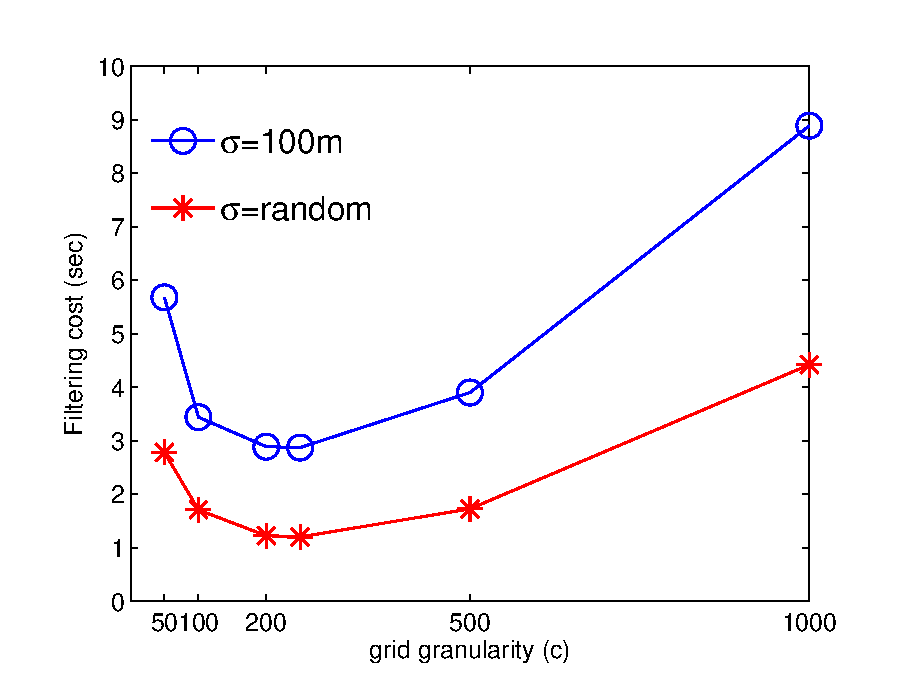
\includegraphics[scale=0.7]{figures/grid_granularity.eps}
\centering
\caption{Κλιμάκωση χρόνου εκτέλεσης για διάφορες υποδιαιρέσεις του καννάβου}	
\label{fig1}
\end{figure} 

Στο Σχήμα~\ref{Quadtree}, παρουσιάζεται ένα παράδειγμα εισαγωγής σχήματος/εικόνας που περιέχεται σε αρχείο pdf, ενώ στο Κεφάλαιο \ref{chap2}, στο Σχήμα \ref{dataconnection} παρουσιάζεται ένα παράδειγμα εισαγωγής σχήματος/εικόνας που περιέχεται σε αρχείο jpg.
\begin{figure}[htb]
\centering
\includegraphics[width = 0.57\columnwidth, height = 8.5cm ]{figures/quadtree.pdf}
\caption{Quadtree partitioning.}
\label{Quadtree}
\end{figure}

\subsection{Σχήματα}
Ακολουθεί στο Σχήμα~\ref{fig2} ένα παράδειγμα σχήματος φτιαγμένου με εντολές του πακέτου Ti\textit{k}Z.
\begin{figure}[htb]
\begin{center}
\begin{tikzpicture}
\draw (-2,0) -- (2,0);
\filldraw [gray] (0,0) circle (2pt);
\draw (-2,-2) .. controls (0,0) .. (2,-2);
%\draw (-2,2) .. controls (-1,0) and (1,0) .. (2,2);
 \draw[gray, thick] (-1,2) -- (2,-4);
\draw[gray, thick] (-1,-1) -- (2,2);
\filldraw[black] (0,0) circle (2pt)  ;
\end{tikzpicture}
\end{center}
\caption{Παράδειγμα σχήματος με εντολές του πακέτου Ti\textit{k}Z}	
\label{fig2}
\end{figure}

\subsection{Μαθηματικές εκφράσεις}
Ακολουθούν παραδείγματα μαθηματικών εκφράσεων.
\begin{eqnarray}
\hat{I}(x,u,t)     &=& dist(y(t_f),\Gamma)
+  \int_t^{t_f} \: {\cal L}( y(s),u(s),s) \: ds
\label{con11b}
\end{eqnarray}

     \[
        \frac{d}{dx}\left( \int_{0}^{z} f(u)\,du\right)=f(x).
     \]

\subsection{Αλγόριθμοι}
Ακολουθεί ο Αλγόριθμος~\ref{alg1}, ο οποίος είναι μορφοποιημένος με τα πακέτα algorithm και algorithmic.

\begin{algorithm}[htb]
\caption{\ \ \ Probabilistic $k\theta NN$ Monitoring}
\begin{algorithmic}[1]
\begin{small}

\STATE{\bf Procedure} {\em VerifyCandidate} (focal query point $q$, threshold $\theta$, object $o$, list of auxiliary objects $P$, distance $kMAXDIST$) 

\IF { $\Phi(o, kMAXDIST) \geq \theta$ {\bf and} $L_2(q, o) \leq L_2(q, P.$top()) }

\STATE {$P$.pop()};   \ \ \ \ \ \ \ \ {\em //Replace the most extreme element in $P$, since candidate $o$ ... }

\STATE {$P$.push($o$)};  \ \ \ \ \ {\em //... has enough probability and has its mean closer to focal $q$ }

\ENDIF

\STATE {\bf End Procedure}


\end{small}
\end{algorithmic}
\label{alg1}
\end{algorithm}

\subsection{Θεωρήματα, Πορίσματα, Ορισμοί, κλπ.}

Ακολουθεί παράδειγμα θεωρήματος από την ιστοσελίδα  {\small\url{https://www.overleaf.com/learn/latex/Theorems_and_proofs}}

\begin{theorem}
Let $f$ be a function whose derivative exists in every point, then $f$ 
is a continuous function.
\end{theorem}

\subsection{Απαριθμήσεις}

Μια απαρίθμηση (itemized list) βοηθά στην παρουσίαση μιας σειράς περιπτώσεων με σαφήνεια.
Ακολουθεί παράδειγμα.

H εκπαίδευση στην Ελλάδα διακρίνεται σε:
\begin{itemize}
\item Πρωτοβάθμια 
\item Δευτεροβάθμια 
\item Τριτοβάθμια 
\end{itemize}

\subsection{Είδη πηγών στις αναφορές}

Στο references.bib μπορεί να δει κανείς πώς γράφονται διάφορα είδη πηγών 
(Βιβλία Ξενόγλωσσα \cite{goossens93},
Βιβλία Ελληνικά \cite{greekbook},
Άρθρα σε επιστημονικά περιοδικά \cite{LiArTs13},
Άρθρα σε επιστημονικά συνέδρια \cite{dcis2011},
Ιστοσελίδες \cite{Docker},
Πτυχιακές Εργασίες \cite{elli05},
Διπλωματικές Εργασίες \cite{zoi04},
Μεταπτυχιακές Διπλωματικές Εργασίες \cite{master04},
Διδακτορικές Διατριβές \cite{phd045},
Τεχνικές Αναφορές \cite{MSU-CSE-05-29},
Διπλώματα Ευρεσιτεχνίας \cite{viswanathan2014convenient}),
Κεφάλαια σε συλλογικούς τόμους
\cite{[PS11]}.

	
% % %	
%     \renewcommand{\thechapter}{B}
%     % Παράρτημα B

 
\chapter{Τίτλος 2ου Παραρτήματος\label{appendixB}}

Τα παραρτήματα περιλαμβάνουν συνοδευτικό, υποστηρικτικό υλικό (πίνακες, φωτογραφίες, ερωτηματολόγια, στατιστικά στοιχεία, αποδείξεις, περιγραφές  λογισμικών  προγραμμάτων,  παραδείγματα,  περιγραφές 
πολύπλοκων διαδικασιών, λίστα με πρωτογενή στοιχεία, λεπτομερής περιγραφή και προδιαγραφές εξοπλισμού, οδηγίες εγκατάστασης λογισμικού, κ.λπ.), ή αλλιώς ό,τι θεωρείται χρήσιμο να περιγραφεί, αλλά δεν συνηθίζεται να 
εντάσσεται μέσα στο κυρίως κείμενο της Εργασίας.  Στο κυρίως κείμενο της Εργασίας πρέπει να γίνονται οι κατάλληλες παραπομπές προς τα παραρτήματα, όπου το κείμενο σχετίζεται με υλικό που περιλαμβάνεται σε αυτά. Ένα παράρτημα, αναλόγως με το περιεχόμενό του, μπορεί να είναι ενιαίο, ή να χωρίζεται σε ενότητες.

% % Εάν υπάρχει μόνο ένα Παράρτημα,
% % μπαίνουν σε σχόλια οι παραπάνω γραμμές 
% % και ρυθμίζεται αρίθμηση χωρίς γράμμα
% %   \renewcommand{\thechapter}{} 
% %   \renewcommand{\thesection}{\arabic{section}}
% %
% % Ακολουθεί αρχείο μεμονωμένου Παραρτήματος
% % (διαφορετική δομή από appA/appΒ)
% %   % Μεμονωμένο Παράρτημα 
% ορίζεται ο τίτλος του παραρτήματος
\edef\chaptertitle{Τίτλος Παραρτήματος}
\label{appendix}

% Μην τροποποιήσετε τις ακόλουθες εντολές
\chapter*{\chaptername\\\vspace{1cm} \chaptertitle} 
\addcontentsline{toc}{chapter}{\chaptername\texorpdfstring{\\}~\chaptertitle}
\setcounter{section}{0}
\renewcommand{\chaptermark}[1]{\markboth{\textit{\chaptername. \chaptertitle}}{}}
\chaptermark{}


Τα παραρτήματα περιλαμβάνουν συνοδευτικό, υποστηρικτικό υλικό (πίνακες, φωτογραφίες, ερωτηματολόγια, στατιστικά στοιχεία, αποδείξεις, περιγραφές  λογισμικών  προγραμμάτων,  παραδείγματα,  περιγραφές 
πολύπλοκων διαδικασιών, λίστα με πρωτογενή στοιχεία, λεπτομερής περιγραφή και προδιαγραφές εξοπλισμού, οδηγίες εγκατάστασης λογισμικού, κ.λπ.), ή αλλιώς ό,τι θεωρείται χρήσιμο να περιγραφεί, αλλά δεν συνηθίζεται να 
εντάσσεται μέσα στο κυρίως κείμενο της Εργασίας.  Στο κυρίως κείμενο της Εργασίας πρέπει να γίνονται οι κατάλληλες παραπομπές προς τα παραρτήματα, όπου το κείμενο σχετίζεται με υλικό που περιλαμβάνεται σε αυτά. Ένα παράρτημα, αναλόγως με το περιεχόμενό του, μπορεί να είναι ενιαίο, ή να χωρίζεται σε ενότητες.


\section{Δυνατότητες του \LaTeX}

Kαθώς το παρόν αποτελεί ένα πρότυπο συγγραφής διπλωματικών εργασιών, στην ενότητα αυτή επιδεικνύονται ορισμένες από τις δυνατότητες το \LaTeX οι οποίες μπορούν να αξιοποιηθούν στο κείμενο μιας διπλωματικής εργασίας (μια καλή πηγή για τη διερεύνηση των δυνατοτήτων του \LaTeX είναι η ιστοσελίδα {\small\url{https://www.overleaf.com/learn/latex/Main_Page}}).

\subsection{Πίνακες}
Ο Πίνακας~\ref{tab1} είναι ένα παράδειγμα πίνακα σχεδιασμένου με εντολές του περιβάλλοντος \texttt{tabular}.
\begin{table}[htb]
\centering
\caption{Παράμετροι πειραμάτων}
\label{tab1}
\begin{tabular}{|c|>{\centering\arraybackslash}m{8cm}|}
\hline Πλήθος κελιών καννάβου \textit{{c}} $\times$ \textit{{c}} & 50 $\times$ 50, 100 $\times$ 100, 200 $\times$ 200, \textbf{250} $\times$ \textbf{250}, 500 $\times$ 500, 1000 $\times$ 1000  \\
\hline Τυπική απόκλιση $\sigma$ & 25{m}, 50{m}, 75{m}, \textbf{100{m}}, 150{m}, 200{m} \\
\hline Αριθμός εγγύτερων γειτόνων \textit{{k}} & 1, 2, \textbf{3}, 4, 5, 10, 20 \\
\hline Πιθανοτικό κατώφλι $\theta$ & 50$\%$, 60$\%$, 70$\%$, \textbf{75$\%$}, 80$\%$, 90$\%$, 99$\%$ \\
\hline  
\end{tabular}

\end{table}

\subsection{Διαγράμματα - Γραφικές παραστάσεις}
Στο Σχήμα~\ref{fig1}, παρουσιάζεται ένα παράδειγμα γραφικής παράστασης σχεδιασμένης με το Gnuplot.
\begin{figure}[htb]
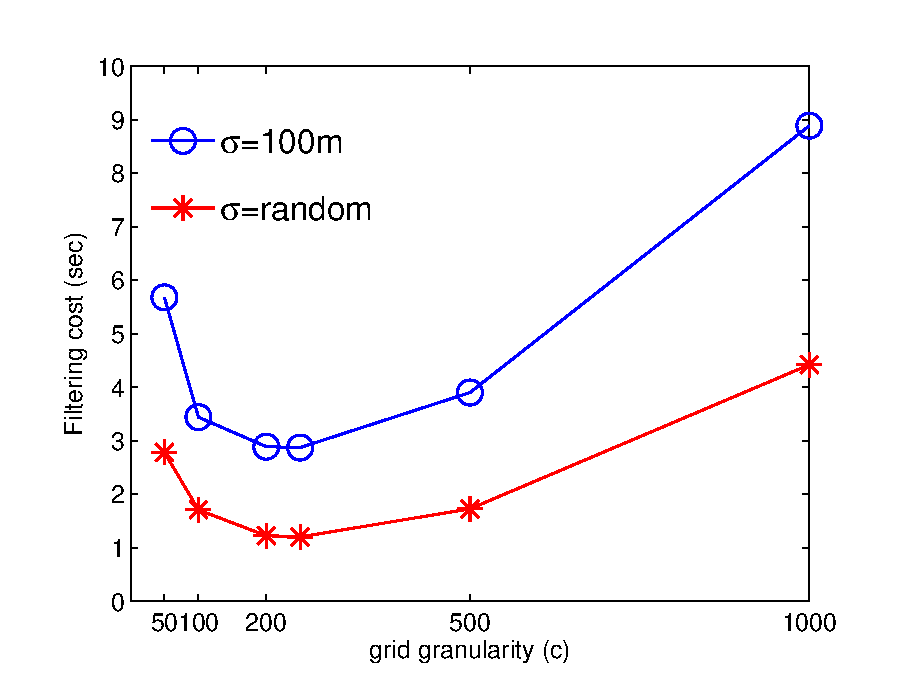
\includegraphics[scale=0.7]{figures/grid_granularity.eps}
\centering
\caption{Κλιμάκωση χρόνου εκτέλεσης για διάφορες υποδιαιρέσεις του καννάβου}	
\label{fig1}
\end{figure} 

\subsection{Σχήματα}
Ακολουθεί στο Σχήμα~\ref{fig2} ένα παράδειγμα σχήματος φτιαγμένου με εντολές του πακέτου Ti\textit{k}Z.
\begin{figure}[htb]
\begin{center}
\begin{tikzpicture}
\draw (-2,0) -- (2,0);
\filldraw [gray] (0,0) circle (2pt);
\draw (-2,-2) .. controls (0,0) .. (2,-2);
%\draw (-2,2) .. controls (-1,0) and (1,0) .. (2,2);
 \draw[gray, thick] (-1,2) -- (2,-4);
\draw[gray, thick] (-1,-1) -- (2,2);
\filldraw[black] (0,0) circle (2pt)  ;
\end{tikzpicture}
\end{center}
\caption{Παράδειγμα σχήματος με εντολές του πακέτου Ti\textit{k}Z}	
\label{fig2}
\end{figure}

\subsection{Αλγόριθμοι}
Ακολουθεί ο Αλγόριθμος~\ref{alg1}, ο οποίος είναι μορφοποιημένος με τα πακέτα algorithm και algorithmic.

\begin{algorithm}[htb]
\caption{\ \ \ Probabilistic $k\theta NN$ Monitoring}
\begin{algorithmic}[1]
\begin{small}

\STATE{\bf Procedure} {\em VerifyCandidate} (focal query point $q$, threshold $\theta$, object $o$, list of auxiliary objects $P$, distance $kMAXDIST$) 

\IF { $\Phi(o, kMAXDIST) \geq \theta$ {\bf and} $L_2(q, o) \leq L_2(q, P.$top()) }

\STATE {$P$.pop()};   \ \ \ \ \ \ \ \ {\em //Replace the most extreme element in $P$, since candidate $o$ ... }

\STATE {$P$.push($o$)};  \ \ \ \ \ {\em //... has enough probability and has its mean closer to focal $q$ }

\ENDIF

\STATE {\bf End Procedure}


\end{small}
\end{algorithmic}
\label{alg1}
\end{algorithm}

\subsection{Μαθηματικές εκφράσεις}
Ακολουθούν παραδείγματα μαθηματικών εκφράσεων.
\begin{eqnarray}
\hat{I}(x,u,t)     &=& dist(y(t_f),\Gamma)
+  \int_t^{t_f} \: {\cal L}( y(s),u(s),s) \: ds
\label{con11b}
\end{eqnarray}

     \[
        \frac{d}{dx}\left( \int_{0}^{z} f(u)\,du\right)=f(x).
     \]

\subsection{Θεωρήματα, Πορίσματα, Ορισμοί, κλπ.}

Ακολουθεί παράδειγμα θεωρήματος από την ιστοσελίδα  {\small\url{https://www.overleaf.com/learn/latex/Theorems_and_proofs}}

\begin{theorem}
Let $f$ be a function whose derivative exists in every point, then $f$ 
is a continuous function.
\end{theorem}

\subsection{Απαριθμήσεις}

Μια απαρίθμηση (itemized list) βοηθά στην παρουσίαση μιας σειράς περιπτώσεων με σαφήνεια.
Ακολουθεί παράδειγμα.

H εκπαίδευση στην Ελλάδα διακρίνεται σε:
\begin{itemize}
\item Πρωτοβάθμια 
\item Δευτεροβάθμια 
\item Τριτοβάθμια 
\end{itemize}

\subsection{Είδη πηγών στις αναφορές}

Στο references.bib μπορεί να δει κανείς πώς γράφονται διάφορα είδη πηγών 
(Βιβλία Ξενόγλωσσα \cite{goossens93},
Βιβλία Ελληνικά \cite{greekbook},
Άρθρα σε επιστημονικά περιοδικά \cite{LiArTs13},
Άρθρα σε επιστημονικά συνέδρια \cite{dcis2011},
Ιστοσελίδες \cite{LaTeXProject},
Πτυχιακές Εργασίες \cite{elli05},
Διπλωματικές Εργασίες \cite{zoi04},
Μεταπτυχιακές Διπλωματικές Εργασίες \cite{master04},
Διδακτορικές Διατριβές \cite{phd045},
Τεχνικές Αναφορές \cite{MSU-CSE-05-29},
Διπλώματα Ευρεσιτεχνίας \cite{viswanathan2014convenient}),
Κεφάλαια σε συλλογικούς τόμους
\cite{[PS11]}.

 

% %
%%%%%%%%%%%%%%%%%%%%%%%%%%%%%%%%%%%%%%%%%%%%%%%%%%%%


\end{document}